\section{Data Acquisition}
\label{sec:data_acquisition}

The dataset used for this study comes from the Inside Airbnb website
\textcite{Airbnb}. This independent initiative collects Airbnb data for more than 30
major cities around the world that scrapes Airbnb listings, reviews, and
calendar data from multiple cities worldwide. The dataset  was scraped on
December 4, 2019, contains information about the location (latitude and
longitude coordinates) of all Airbnb listings in New York City and data about
the hostname and ID, room type, price, minimum nights, number of reviews
listings per host, and availability...

The raw data is quite untidy and has some weaknesses. The major one is that it
only includes the advertised price (sometimes called the ‘sticker’ price). The
sticker price is the overall nightly price advertised to potential renters,
rather than the actual average amount paid per night by previous guests. A host
can set the advertised prices to any arbitrary amount, and those that do not
have much experience with Airbnb will often set these to unreasonable prices,
such as too low (e.g., \$0) or very high (e.g., \$10,000) amounts.

These variables are listed and defined in Table ~\ref{tab:variable-list}.

\section{Data Preprocessing }
\label{sec:data_cleaning}

Real-world data is often dirty; that is, it is in need of being cleaned up
before it can be used for the desired purpose such as visualization, model
building. This is often called data pre-processing.
Since there are several reasons why data could be “dirty,” there are just as
various techniques to “clean” it.  For this analysis, we will take a look at
three key methods that illustrate ways in which data may be “cleaned,” or better
organized, or scrubbed of potentially incorrect, incomplete, or duplicated data.

\subsection{Data Filtering}

Following \textcite{wang2017price}, this study filtered the listings with at
least one online customer review to guarantee that our sample listings were
"active." This view is supported by \textcite{ye2009impact}  which confirms that online
review ratings are associated with hotel-room sales, indicating that reviews
suggest real transactions.

\subsection{Removing Predictors}

There are three reasons why we should consider removing predictors before
modeling. First, fitting a model with fewer predictors reduces computational
time and complexity. Second, removing highly correlated features makes the model
more parsimonious and interpretable model.  Lastly, some models can be crippled
by predictors with degenerate distributions.  Therefore, eliminating the
problematic predictors prior to fitting a model can significantly improve model
performance and stability.
\begin{itemize}

    \item We remove  predictors with a single unique value as they are  zero
        variance predictors. These predictors are \texttt{has\_availability},
        \texttt{host\_has\_profile\_pic},\texttt{requires\_license},
        \texttt{is\_business\_travel\_ready},
        \texttt{require\_guest\_phone\_verification},\newline
        \texttt{require\_guest\_profile\_picture} (See
        \ref{fig:histogram-feature-distribution}) .
    \item It is beyond the scope of this study to explore the natural language
        processing for predictive modeling.  Therefore,  we will drop free-text
        columns for now, as will other columns that are not useful for
        predicting price (e.g., \texttt{url}, \texttt{hostname}, and other host-related features
        unrelated to the property).

    \item We drop feature which  adds relatively little information, or are
        relative unhelpful in differentiating between different listings.

\end{itemize}

\subsection{Dealing with Missing Values}

Missing data is a common issue in many data analysis applications.  Data may be
missing due to problems with the process of collecting data or equipment
malfunction. Some data may get lost due to system or human error while storing
or transferring the data.

There are two approaches we take to handle missing
data:
\begin{enumerate}
    \item Filling out missing value :  we drop the predictors
        that contain a majority of null entries as in Table
        ~\ref{tab:missing-value}.
    \item Filling in missing value:we perform data imputation, which means
        filling the missing data with some estimated ones. In particular,

        \begin{itemize}

            \item Missing values in numeric features such as the number of
                bathrooms (\texttt{bathrooms}) bathrooms, the number of bedrooms
                (\texttt{bedrooms}), the number of beds (\texttt{beds}) will be
                replaced with the median.

            \item For monetary features such as the amount required as a
                security deposit (\texttt{security\_deposit}), the amount of the cleaning
                fee (\texttt{cleaning\_fee}), the price per additional guest
                (extra\_people), having a missing value for them is the same as
                having the value of \$0, so the missing values will be replaced
                with 0. Similarly, an amenity that has a missing value will be replaced with 0.

        \end{itemize}
\end{enumerate}

\begin{table}[htp]
    \centering
    \caption{Columns with majority of null values}
    \label{tab:missing-value}
{\small
\begin{tabular}{lrr}
\toprule
{} &  count &  percentage \\
\midrule
host\_acceptance\_rate &  50599 &      100.00 \\
jurisdiction\_names   &  50583 &       99.97 \\
license              &  50577 &       99.96 \\
square\_feet          &  50213 &       99.24 \\
monthly\_price        &  45683 &       90.28 \\
weekly\_price         &  44945 &       88.83 \\
\bottomrule
\end{tabular}
}
\end{table}

\subsection{Feature Construction}

\begin{itemize}

    \item We convert DateTime columns such as the date that the host first joined Airbnb
        (\texttt{host\_since}) to measure the number of days a host has been on
        the platform, measured from the date that the data was collected
        (\texttt{host\_days\_active}).

    \item We create a new feature that measures the number of days between the first
        review and  the date we collect the data
        (\texttt{time\_since\_first\_review}) from
        the feature the date of the first review (\texttt{first\_review}).

    \item We can compute the number of days between the most recent review and
        the date the data was scraped (\texttt{time\_since\_last\_review}) using the date of the
        most recent review (\texttt{last\_review}).
\end{itemize}

\subsection{Binning Predictors}

We want to discretize continuous data into "bins" for analysis in many situations, especially when that data has a wide range.
Binning, also known as quantization, is a useful technique for converting continuous numeric features into discrete ones (categories).
In our dataset, we peform the following binning:
\begin{itemize}

    \item The feature that measures proportion of messages that the host replies
(host\_response\_rate) will be bin into four categories '0-49\%', '50-89\%',
'90-99\%', '100\%',

    \item The number of days between the first review and the date we collect the data
        (\texttt{time\_since\_first\_review}) will be bin into '0-6 months', '6-12 months', '1-2
    years', '2-3 years', '4+ years'

    \item The number of days between the most recent review and the date the data was
        scraped (\texttt{time\_since\_last\_review}) will be bin into '0-2 weeks','2-8 weeks',
    '2-6 months', '6-12 months', '1+ year'

    \item Review scores rating (\texttt{review\_scores\_rating}) will be bin into following
        categories '0-79/100', '80-94/100', '95-100/100'
\end{itemize}



\subsection{Data Transformation}

\subsubsection*{Feature Scaling}

Feature scaling is an essential step in the preprocessing process, as some
machine learning algorithms do not perform well when the numerical input
attributes have very different scales.

Feature scaling through standardization (or Z-score normalization) is straightforward and
common-used in the machine learning community.
Standardization means that we rescale the predictors so that they have a zero
mean and standard deviation 1.  We first compute the mean and standard deviation
for the feature and scale it based on:
\[x^{'} = \frac{x - \bar{x}}{\sigma}\]
where $x$ is the original feature vector, $\bar{x} = \textrm{average(x)}$ is the mean of
that feature vector, and $\sigma$ is its standard deviation.

\noindent In our dataset we use  a transformer called StandardScaler from Scikit-Learn for
standardization.

\subsubsection*{Transformation to Resolve Skewness}

Many models assume a normal distribution, which means data are symmetric about
the mean.
Unfortunately, our real-life datasets do not always follow the normal
distribution.  Instead, they are usually skewed, which makes the results of our
statistical analyses invalid.

Figure \ref{fig:histogram-before-transform}
shows the distribution of numerical features. We notice
that most of the predictors have a heavy-tailed distribution. Therefore we
transform them by replacing them with their logarithm. Figure
\ref{fig:histogram-after-transform} shows the result;
some of the distributions become normal. More importantly, the outcome variable
price appears much more normally distributed.

\subsection{Handling Categorical Attributes}

One of the significant problems with machine learning is that many algorithms
cannot work directly with categorical data (non-numerical values).  Hence, we
need a way to convert categorical data into a numerical form, and our machine
learning algorithm can take in that as input. In this study, we use  One-Hot
Encoding, one of the most widely used encoding techniques.  One-hot encoding is
processed in 2 steps:
\begin{enumerate}
    \item First, we split categories into different columns.
    \item We then put 0 for others and 1 as an indicator for the appropriate column.
\end{enumerate}

There is a very simple way to encode the data in python pandas library, using
the \texttt{get\_dummies()} function.

\section{Exploratory Data Analysis}

Before embarking on developing statistical models and generating predictions, it
is essential to understand your data. This is typically done using conventional
numerical and graphical methods. \textcite{tukey1977exploratory} advocated the practice
of exploratory data analysis (EDA) as a critical part of the scientific process.

We present the descriptive statistics of variables in Table
\ref{tab:descriptive-statistic}

\subsection{Numerical Features}
\label{sec:numerical_features}

\subsubsection*{Price}

The nightly advertised prices range from \$0 to \$10,000. The range is so broad
because hosts do not understand how to set Airbnb advertised prices.  Figure
~\ref{fig:price-distribution-1000} and Figure ~\ref{fig:price-distribution-200}
 show the distributions of price up to \$1,000 and \$200 respectively. While the
price's range is extensive, most of its values concentrate on the range \$10 to
\$1000.  Hence, for minimal values under \$10, we will increase them to \$10,
and values above \$1,000 will be reduced to \$1,000.

\begin{figure}[!htbp] \centering
    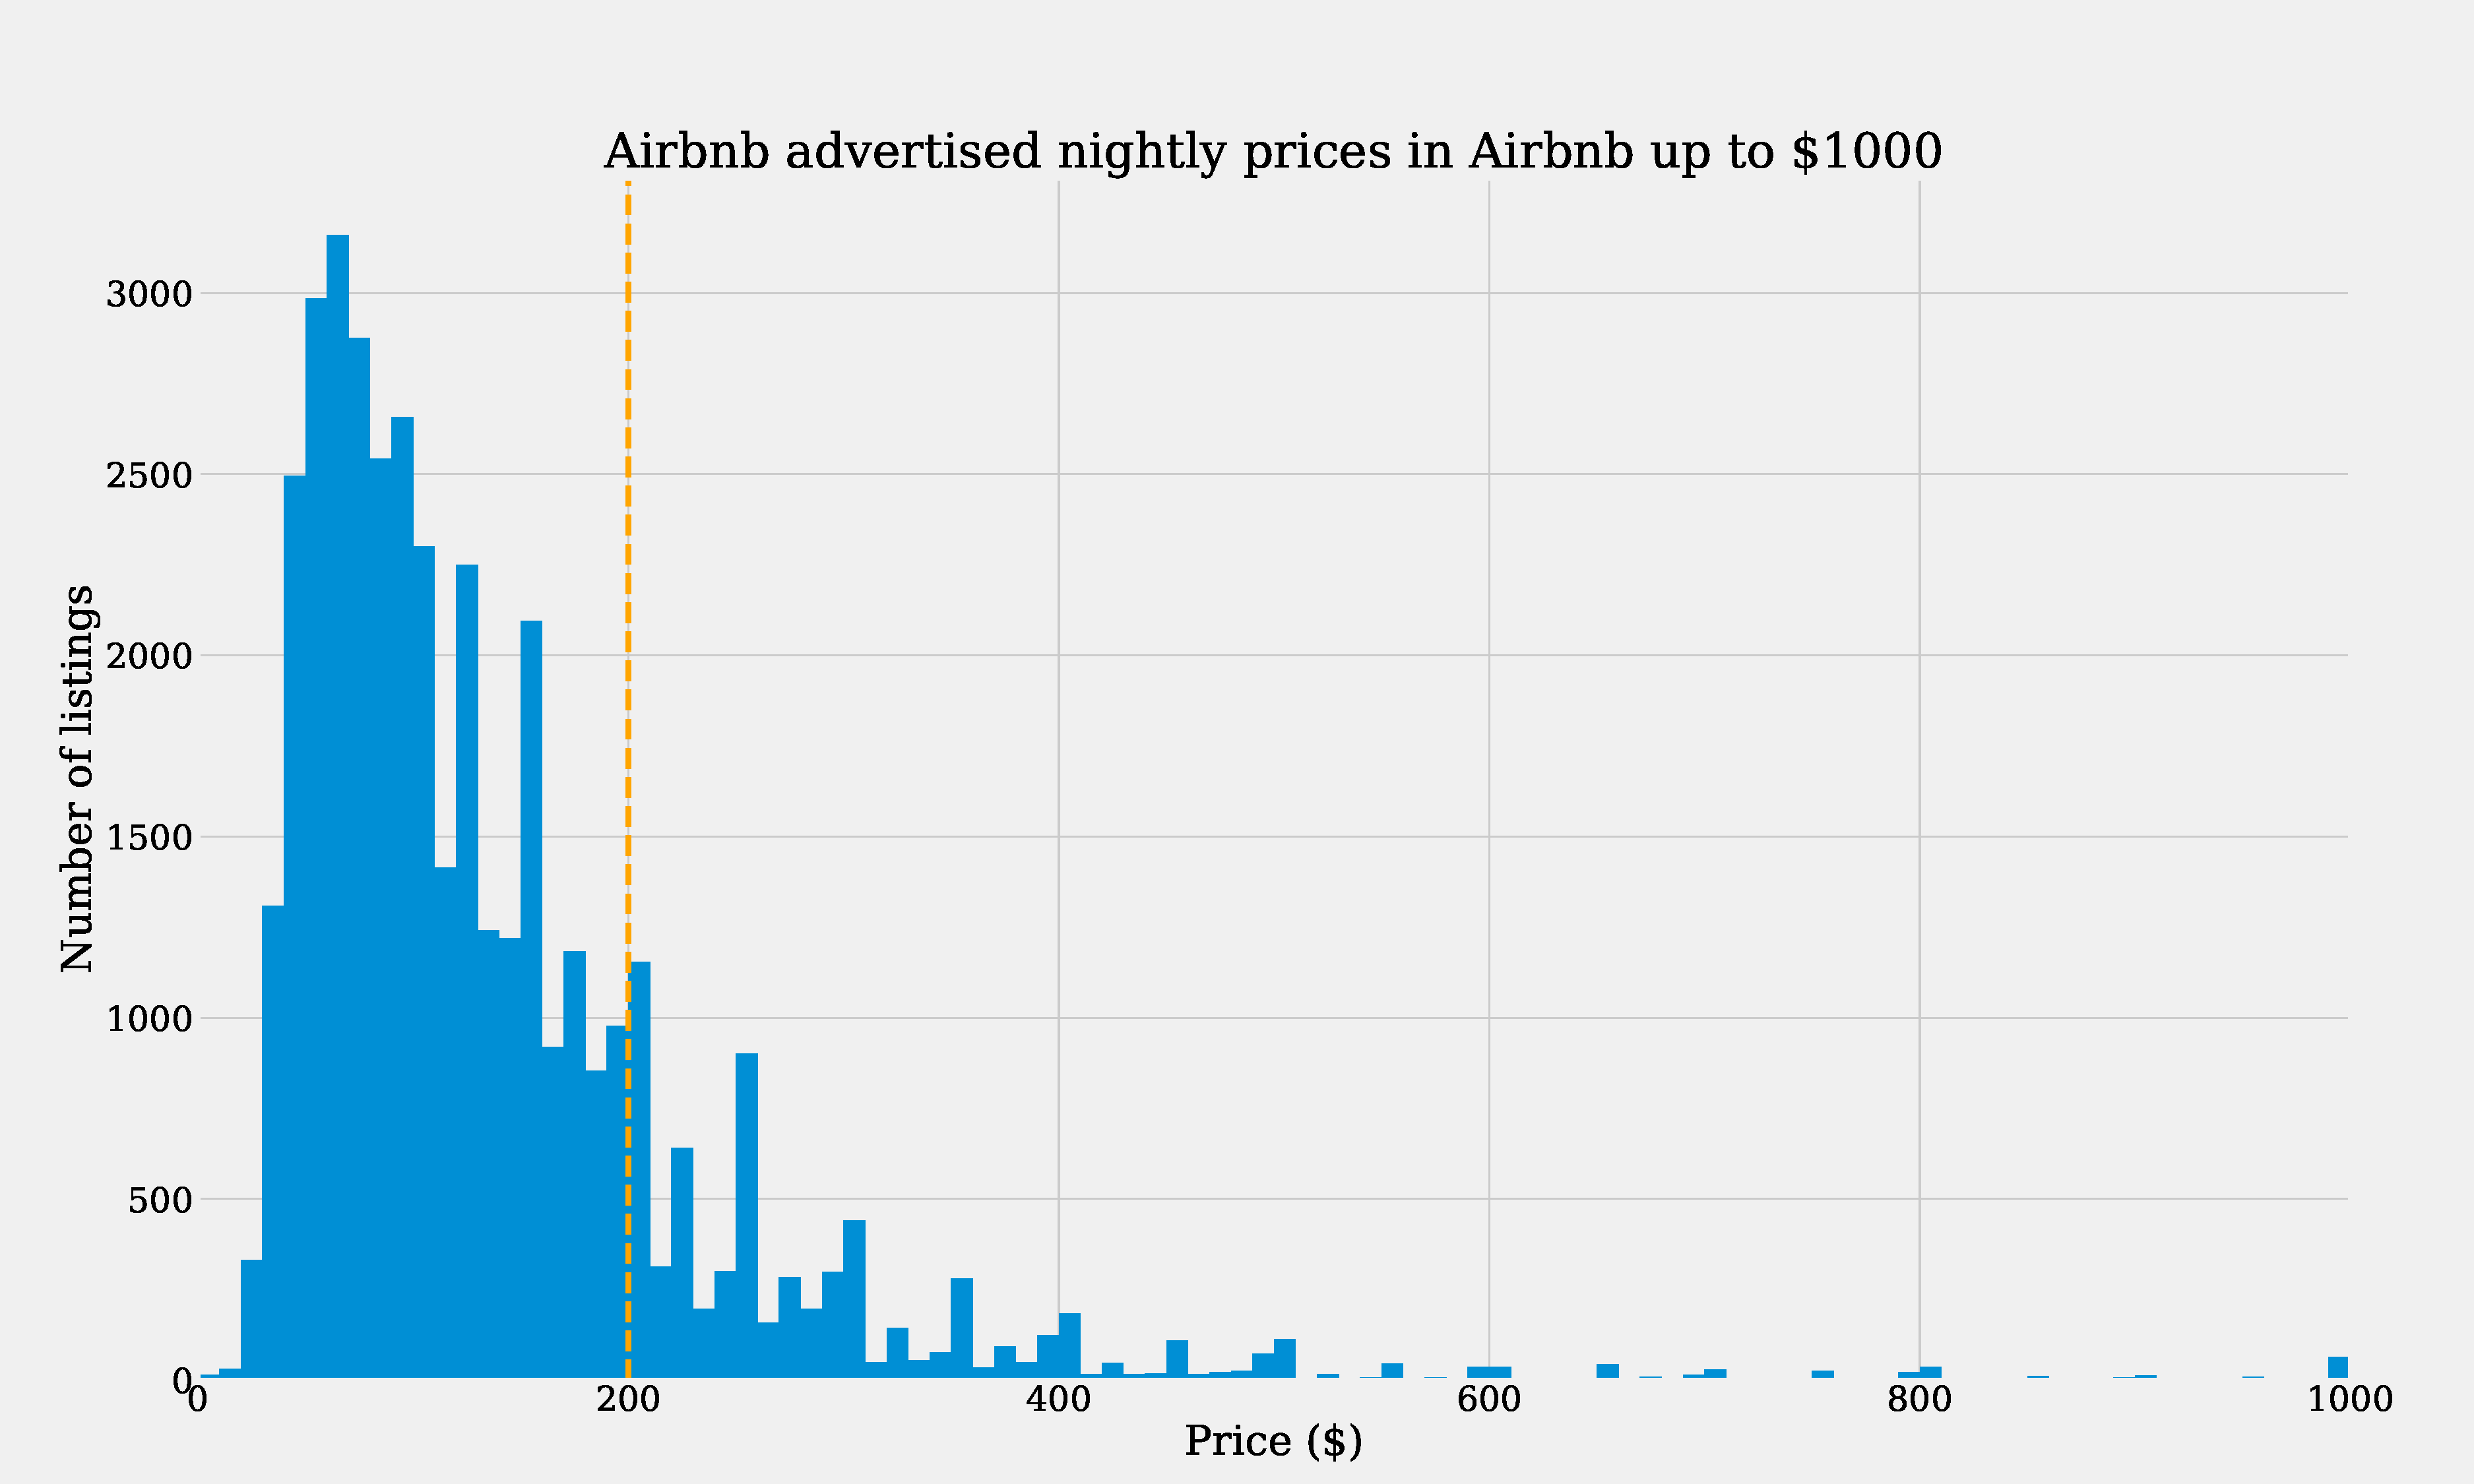
\includegraphics[width=\textwidth]{price-distribution-up-to-1000.pdf}
        \caption{Airbnb advertised price up to \$1000}
        \label{fig:price-distribution-1000}
\end{figure}

\begin{figure}[!htbp] \centering
    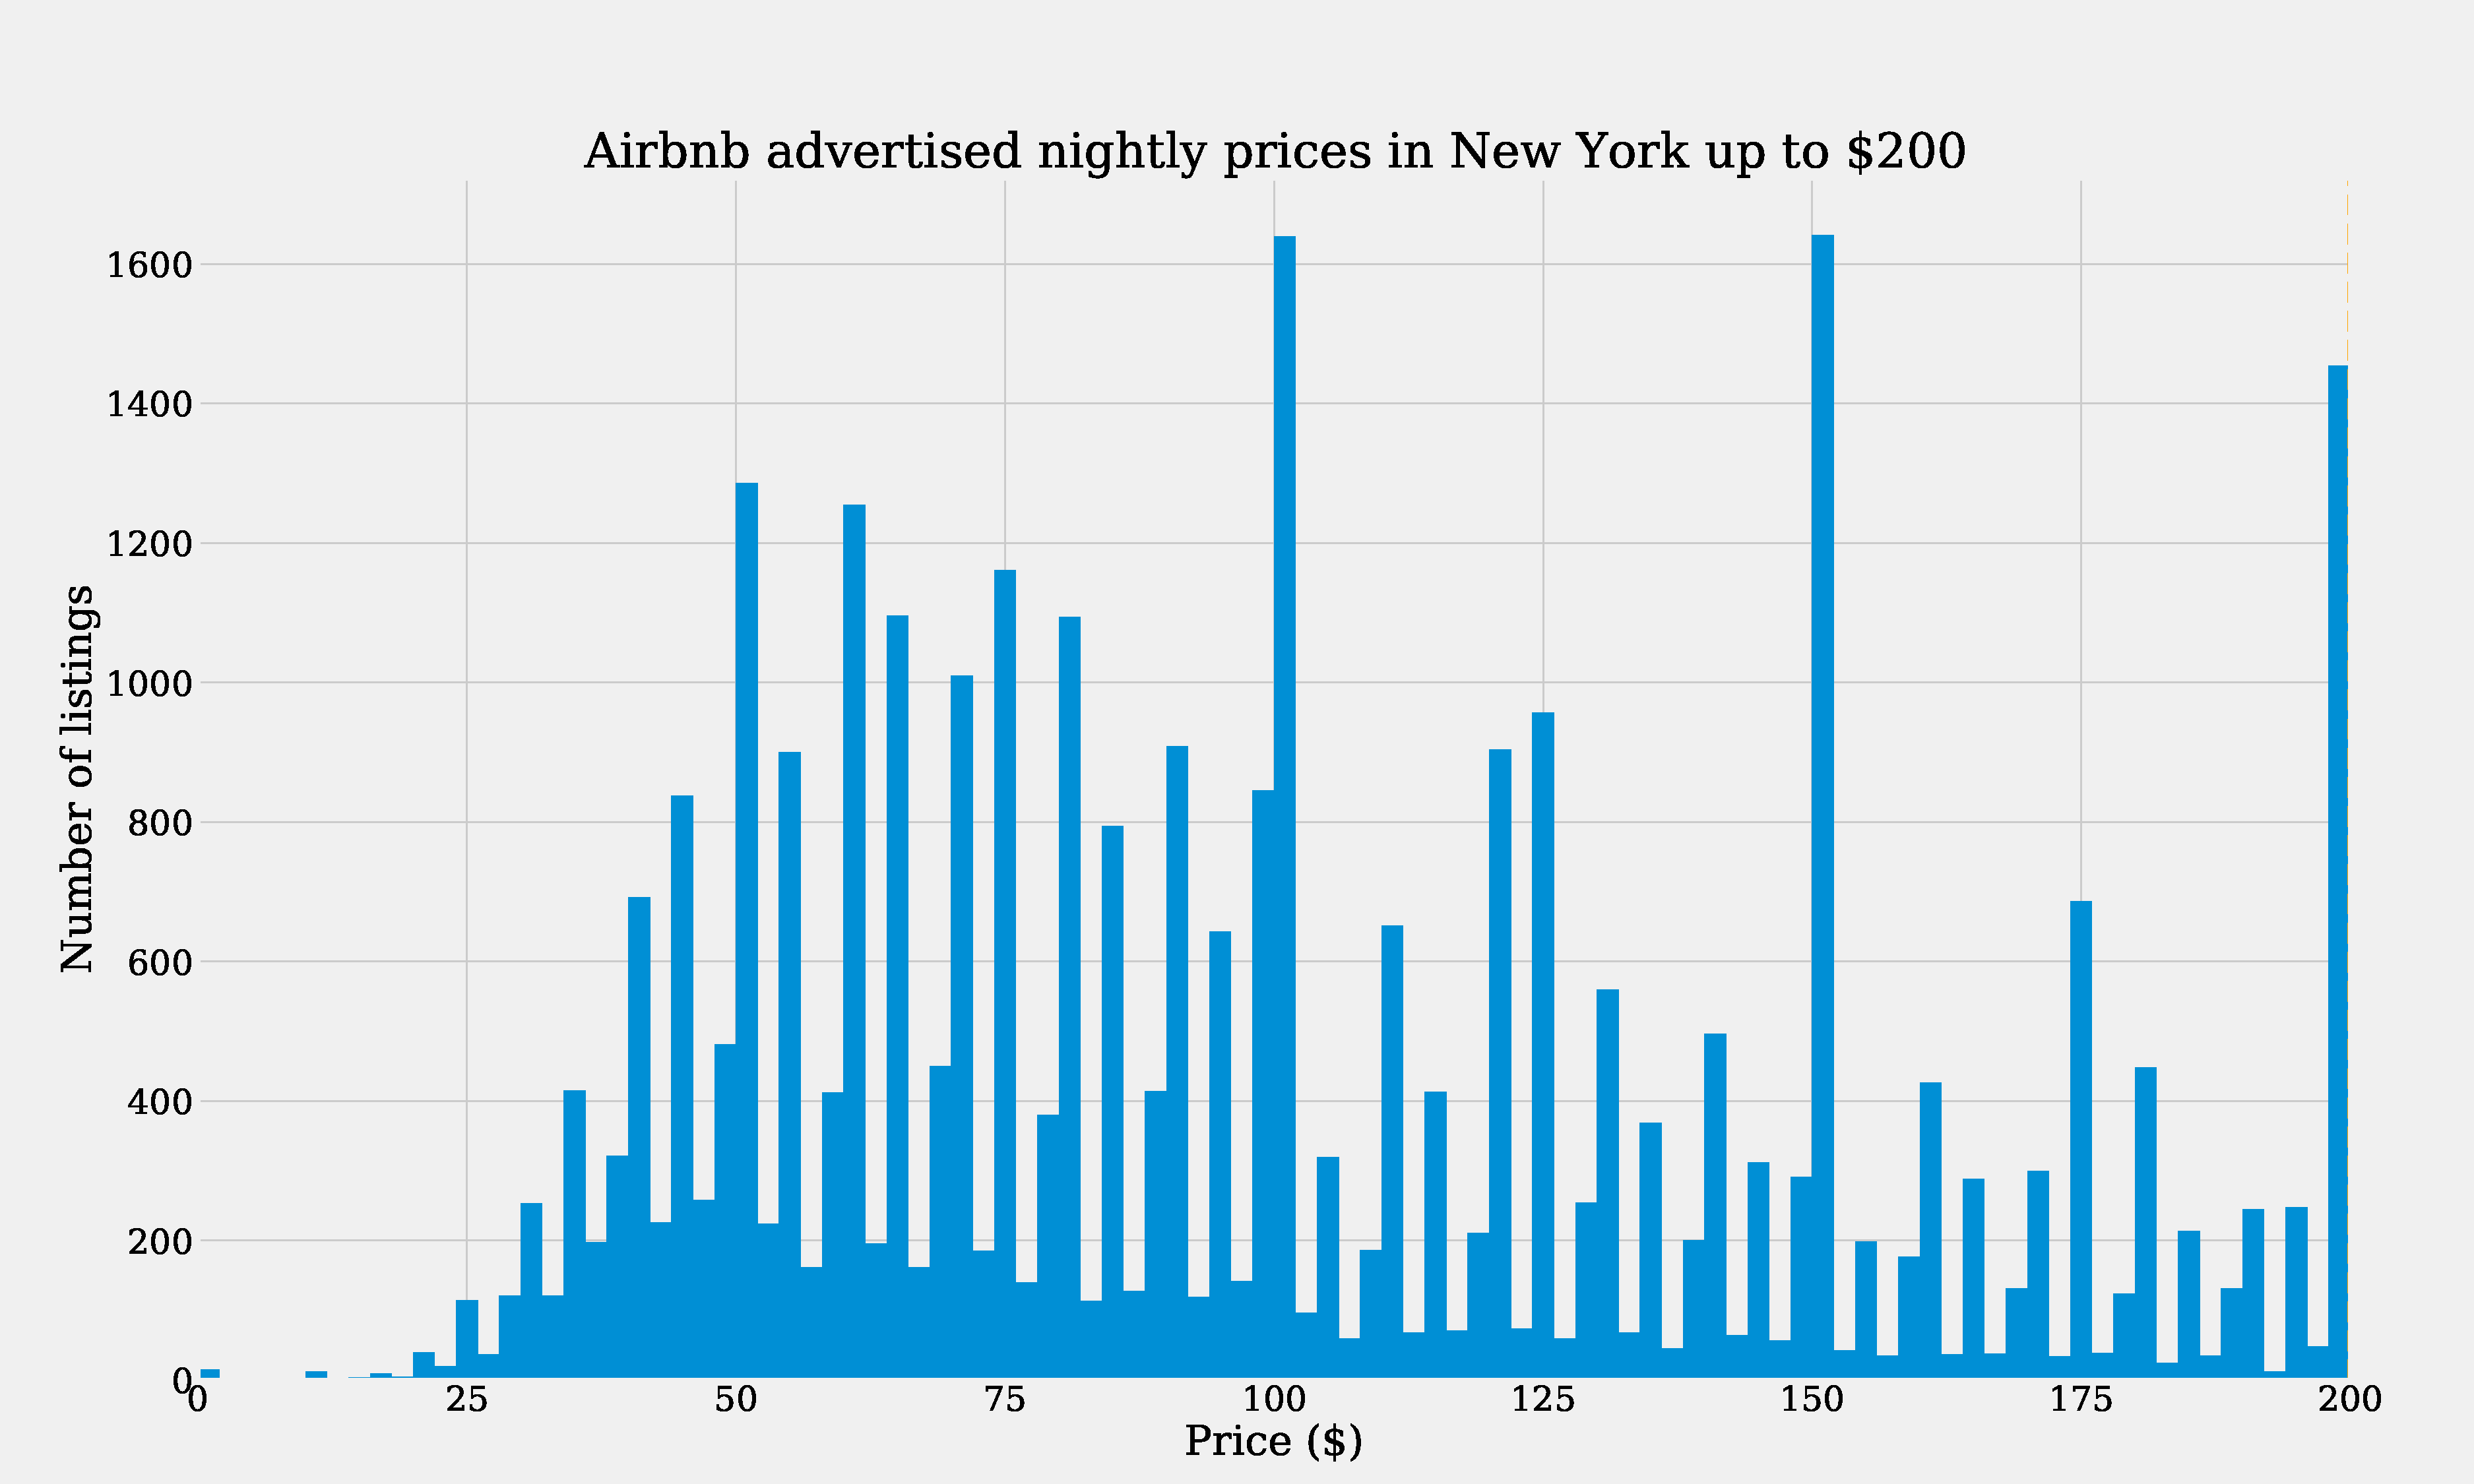
\includegraphics[width=\textwidth]{price-distribution-up-to-200.pdf}
        \caption{Airbnb advertised price up to \$200}
        \label{fig:price-distribution-200}
\end{figure}

\subsubsection*{Host Listings Count}

The median number of listings that the host of each listing has is 1. The mean
is higher (8 in total) due to some hosts running many listings. About 55\% of
listings are from hosts with one listing, and 45\% are from multi-listing hosts.
This feature has been shown to have a positive effect on the price of Airbnb
listings(\cite{chen2017consumer}, \cite{ert2016trust}, \cite{wang2017price})

\subsubsection*{Number of people accommodated, bathrooms, bedrooms and beds}

~\Cref{fig:accommodates-countplot,fig:bathrooms-countplot,fig:bedrooms-countplot,fig:beds-countplot}
  reveal that the most common listing type accommodates two people in one bed
  in one
bedroom with one bathroom.

The number of bedrooms, number of bathrooms, and number of accommodations appear
to have a positive impact on Airbnb rental price (\cite{ert2016trust};
\cite{chen2017consumer}; \cite{wang2017price}; \cite{gibbs2018use}). Figures
\ref{fig:median-price-by-accommodates} - ~\ref{fig:median-price-by-beds} show that the more people a listing
accommodates, the more number of bedrooms it has, the more bathrooms it has, the
higher the price they can charge their customers. However, we can see that those
figures' general trends are similar, which implies that those features may be
highly correlated.

\subsection{Categorical features}
\label{sec:categorical_features}

Our main EDA objective for categorical data is to know the unique values and
their corresponding count.

\subsubsection*{Neighbourhood}
\label{eda:neighbourhood}

Several numbers of published studies recognize the importance of locational
factors in the pricing strategy of Airbnb.  A listing close to the city center
(\cite{gibbs2018use};\cite{li2016pros}; \cite{wang2017price};
\cite{zhang2017key};\cite{gibbs2018use}) and coastline (\cite{perez2018and}) has
a higher room rate.  \cite{perez2018and} also found that a listing located
within sightseeing, eating, or shopping area gains a price premium.

As shown in Figure \ref{fig:borough-number-of-listing} and Figure
\ref{fig:borough-price-distribution}, Manhattan and Brookly have most Airbnb
properties are the most expensive boroughs, which is not surprising because they
are the famous tourist attractions.  In those two boroughs, tourists can find
neighborhoods for almost any interest. For example:

\begin{itemize}
  \item Sightseeing: Midtown is the heart of New York shopping and theater and
    home to some of its most iconic buildings.
  \item Nightlife:  More clubs are found in “Hell’s Kitchen,”
  \item Food: In Soho, tourists can experience a host of the highest-rated
    dining places.
  \item Theather: There is no more convenient home base than
    the Theater District,  located in 42nd Street to 50th Street west of Sixth
    Avenue.
  \item For families: Upper West Side is bordered with parks and playgrounds and
  boasting both a children’s museum and the famed dinosaurs at the American Museum
  of Natural. This neighborhood is also considered one of the safest areas of New
  York City
\end{itemize}


\begin{figure}[!htbp] \centering
  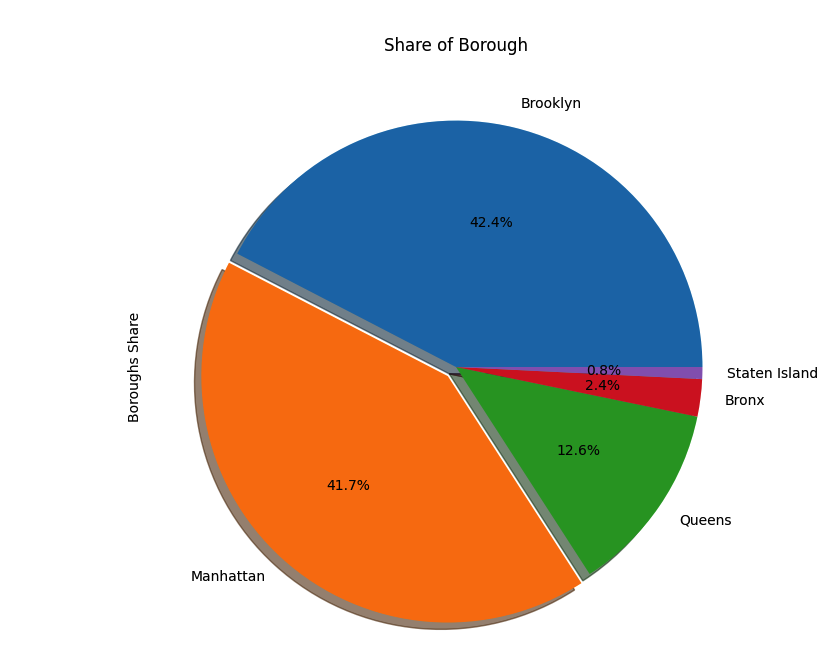
\includegraphics[width=0.9\textwidth]{share-of-borough.png}
    \caption{Borough Listings}
    \label{fig:borough-number-of-listing}
\end{figure}


\begin{figure}[!htbp]\centering
    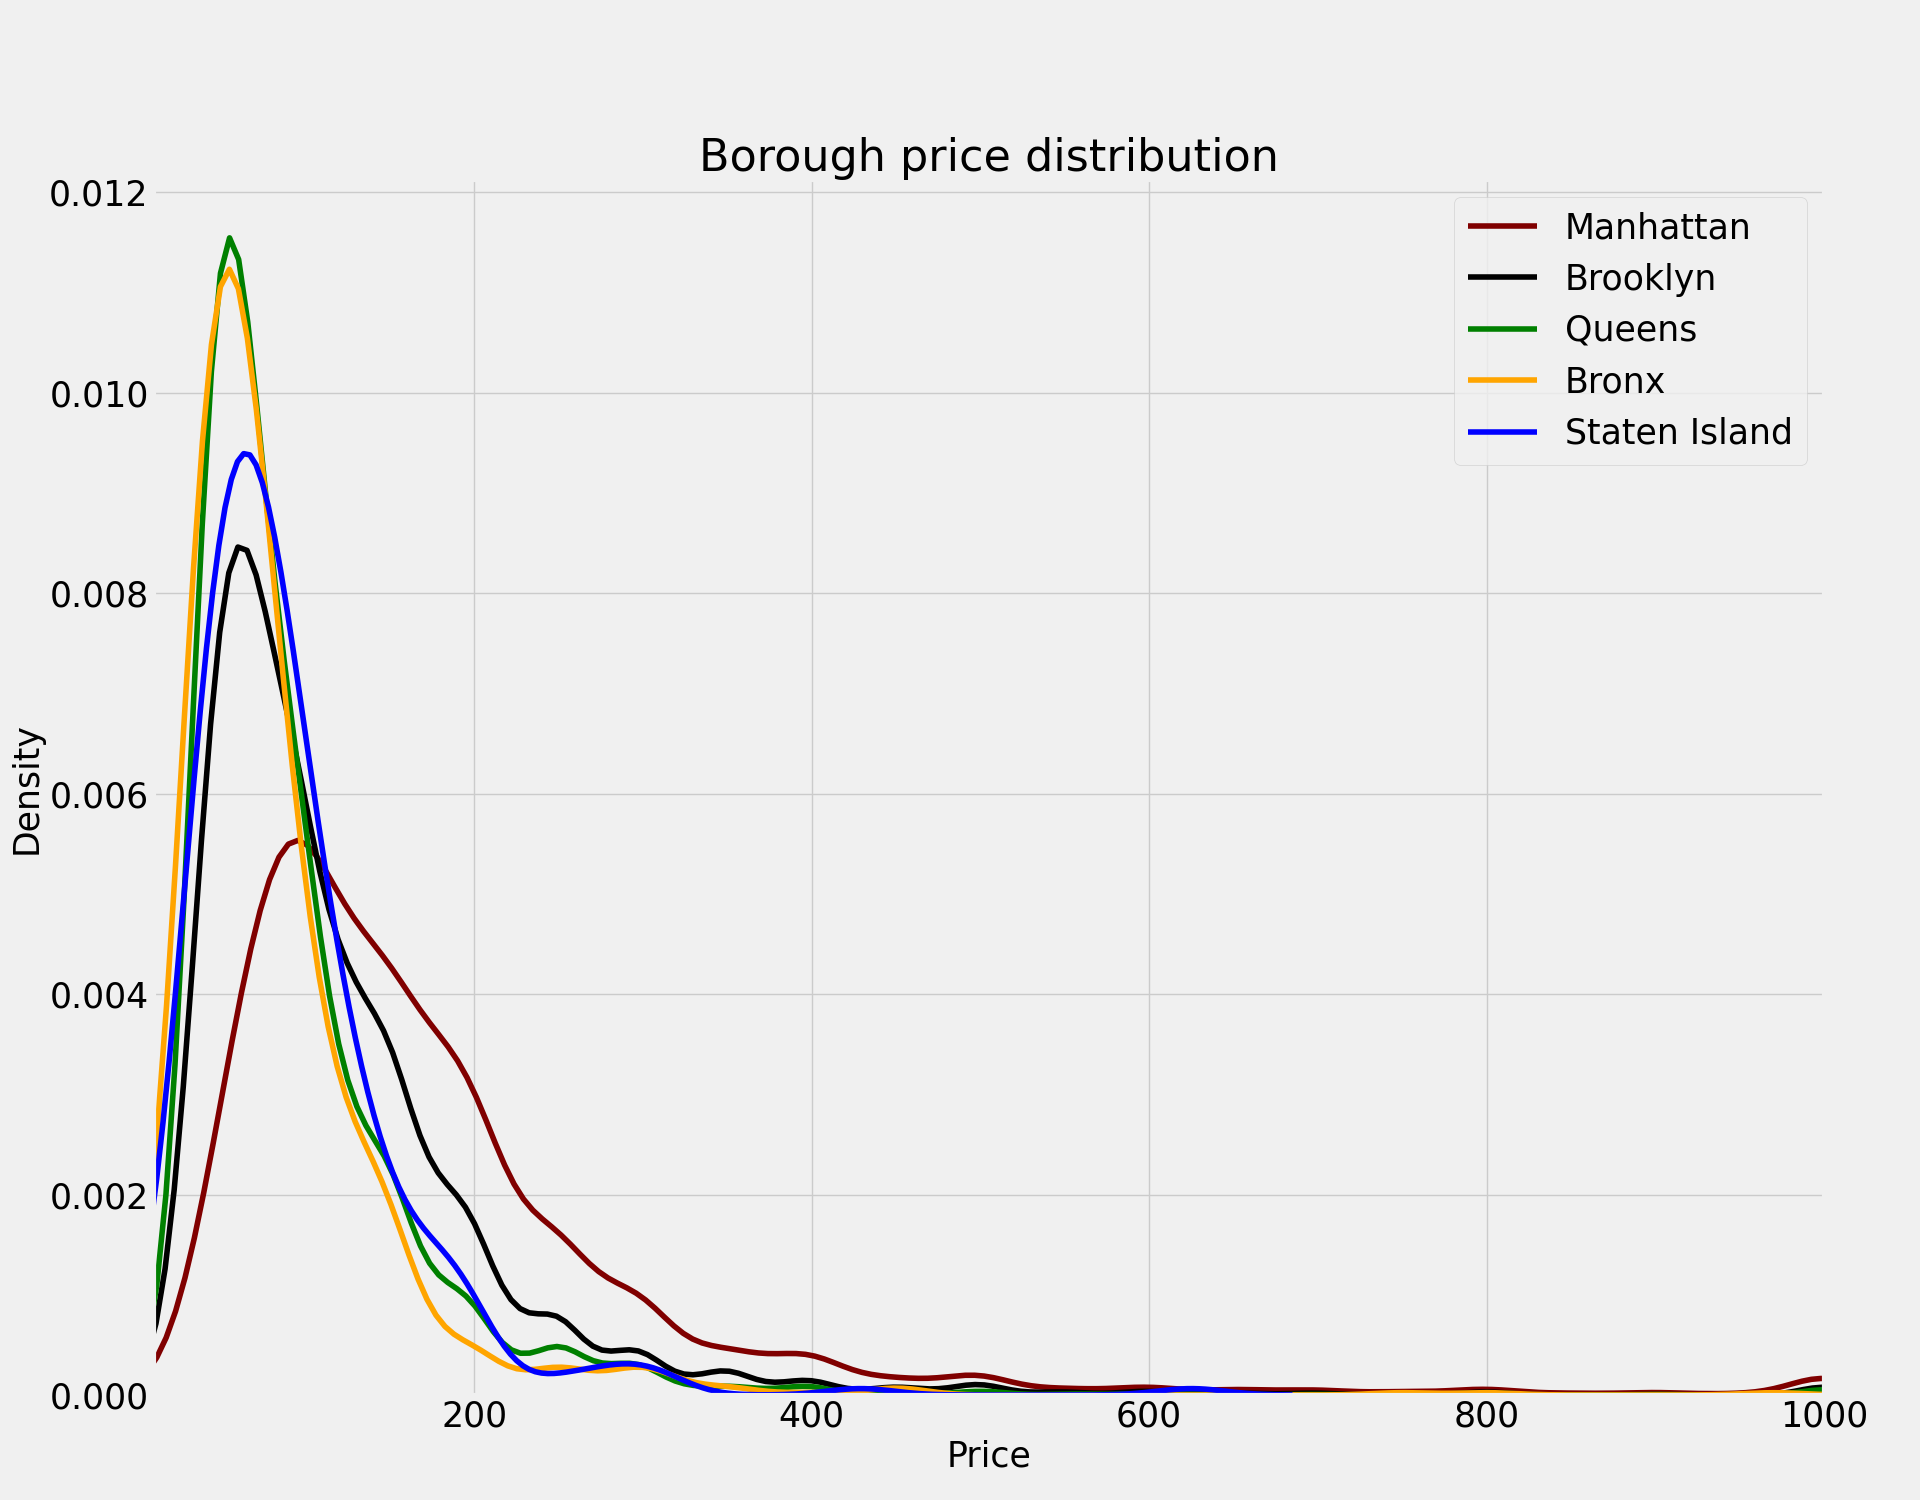
\includegraphics[width=0.9\textwidth]{borough-price-distribution.png}
    \caption{Borough Price Distribution}
    \label{fig:borough-price-distribution}
\end{figure}

\subsubsection*{Property and room types}

As shown in Figure \ref{fig:property_type},
about 80\% properties are apartments. The remainder are houses or more uncommon
property types (e.g. 'bed and breakfast' or 'yurt'). The median price of
apartment type listing is higher than that of house type listing but lower than
uncommon property types (\ref{fig:property_type_price}).

\begin{figure}[!htbp]
    \centering
        \centering
        \caption{Property Type Pie Chart}
        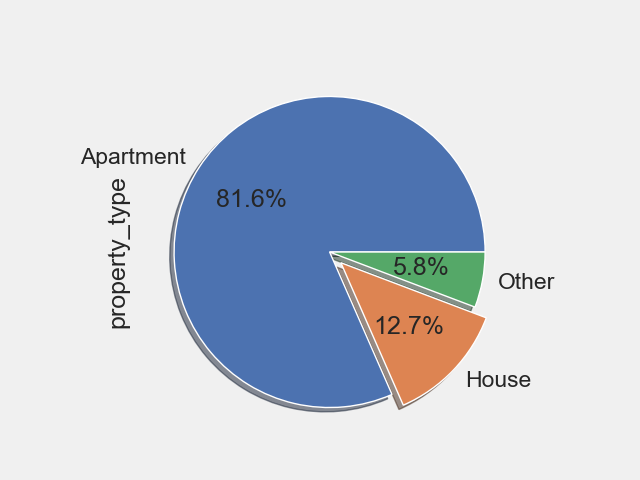
\includegraphics[width=0.7\textwidth]{Figure_12_property_type_pie.png}
      \label{fig:property_type}
\end{figure}

\begin{figure}[!htbp]
        \centering
        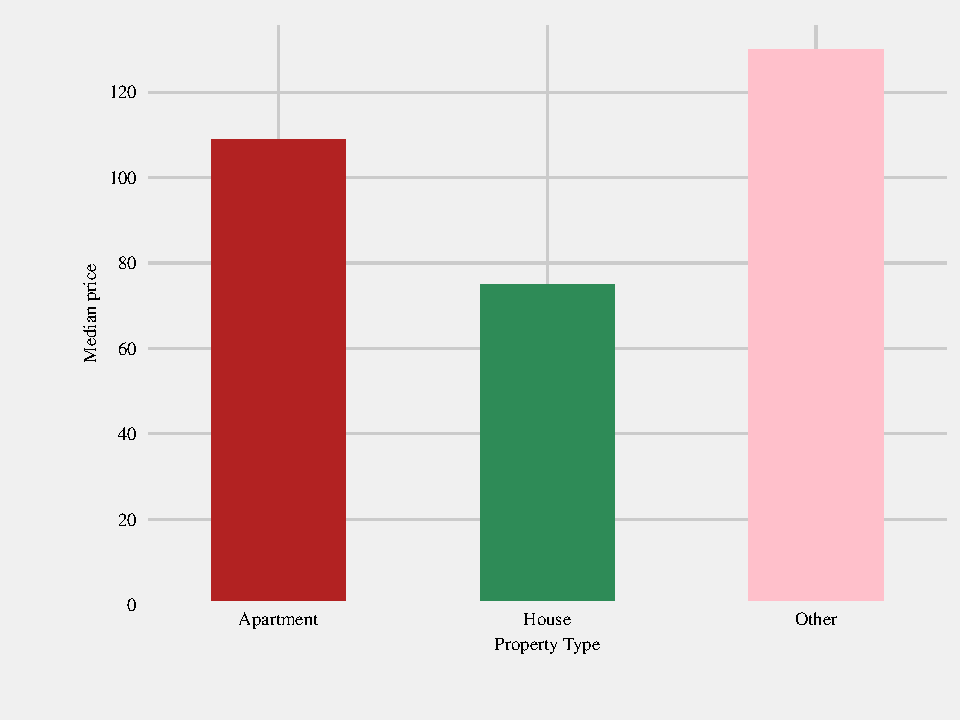
\includegraphics[width=0.85\textwidth]{median-price-by-property-type.pdf}
        \caption{Median Price By Property Type}
        \label{fig:property_type_price}
\end{figure}

Figure ~\ref{fig:room_type_pie} shows that about 52\% of listings are entire homes
(i.e. you are renting the entire property on your own). Most of the remainder
are private rooms (i.e. you are renting a bedroom and possibly also a bathroom,
but there will be other people in the property). Fewer than 3\% are shared rooms
(i.e. you are sharing a room with either the property owner or other guests).

On the question of whether there's a price difference between different types of
rooms, Figure \ref{fig:room_type_price} reveals that the rental price of the
entire home and a private room, and a hotel room is higher than the shared room.
This finding is consistent with many recent studies (\cite{cai2019price} ;
\cite{benitez2018flexible}; \cite{chen2017consumer}; \cite{gibbs2018use})

\begin{figure}[!htbp]
    \centering
        \centering
        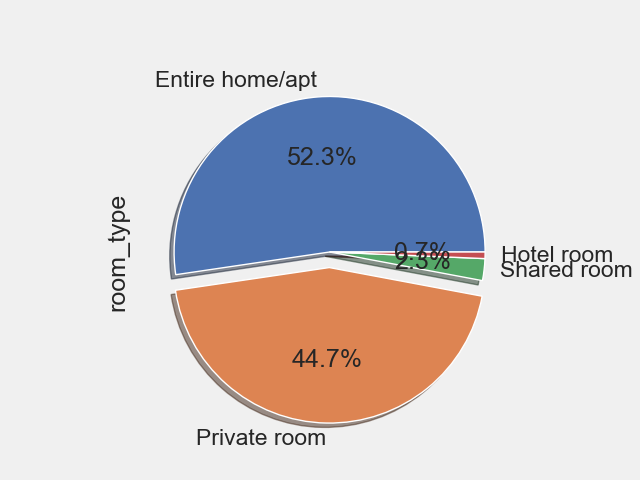
\includegraphics[width=0.7\textwidth]{Figure_12_room_type_pie.png}
        \caption{Room Type Pie Chart}
        \label{fig:room_type_pie}
\end{figure}

\begin{figure}[!htbp]
        \centering
        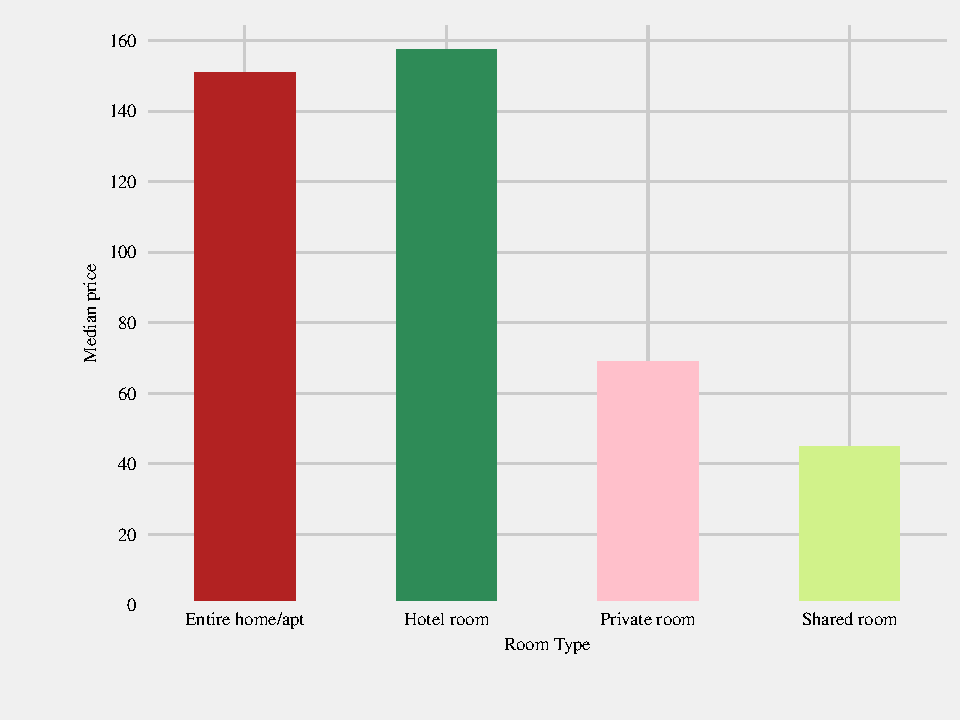
\includegraphics[width=0.85\textwidth]{median-price-by-room-type.pdf}
        \caption{Median Price By Room Type}
        \label{fig:room_type_price}
\end{figure}

\subsubsection*{Reviews}

From Figure   \ref{fig:overall-listing}, we see that, while few listings receive
review ratings of 80 or below, most listings with a review have received a
95-100/100 overall,  indicating that the customers adore their Airbnbs.


As shown in Figure \ref{fig:price_by_review_score_rating}, the review score
rating has a positive effect on the median rental price. It all makes intuitive
sense customers are willing to pay a premium price for a listing with a good
reputation.  However, the evidence for the relationship between is inconclusive.
Many studies (\cite{chen2017consumer}; \cite{gibbs2018use};
\cite{wang2017price}) have shown that the overall rating score has a positive
impact on rental price, while others (\cite{li2016pros}; \cite{zhang2017key})
suggests the otherwise.

\begin{figure}[!htbp]\centering
    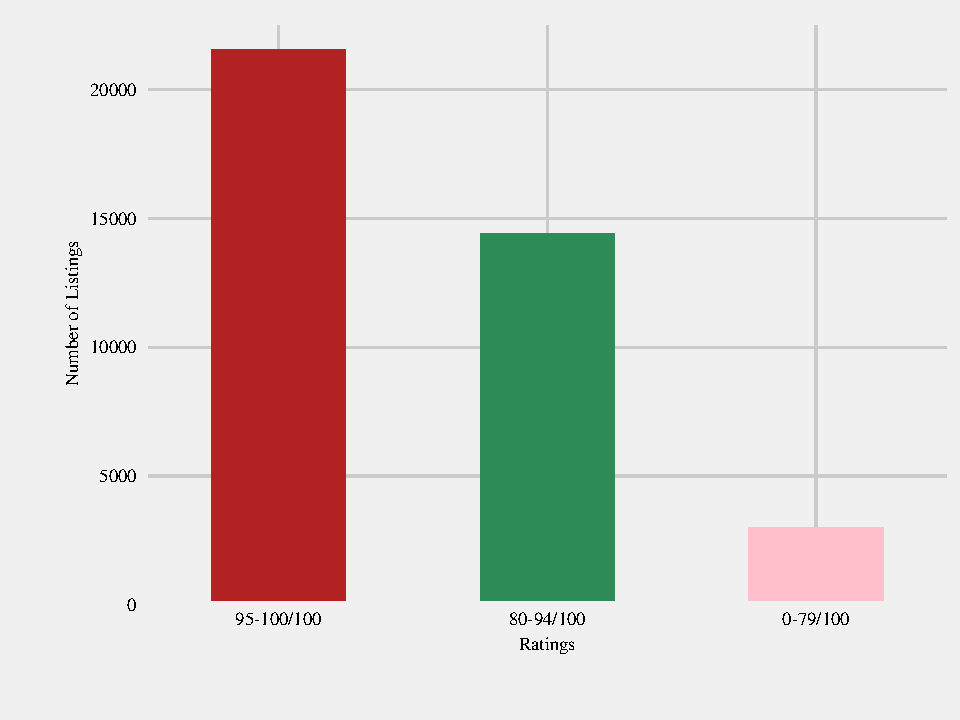
\includegraphics[width=0.85\textwidth]{review-rating-distribution.pdf}
    \caption{Overall Listing Rating Distribution}
    \label{fig:overall-listing}
\end{figure}

\begin{figure}[!htbp]\centering
    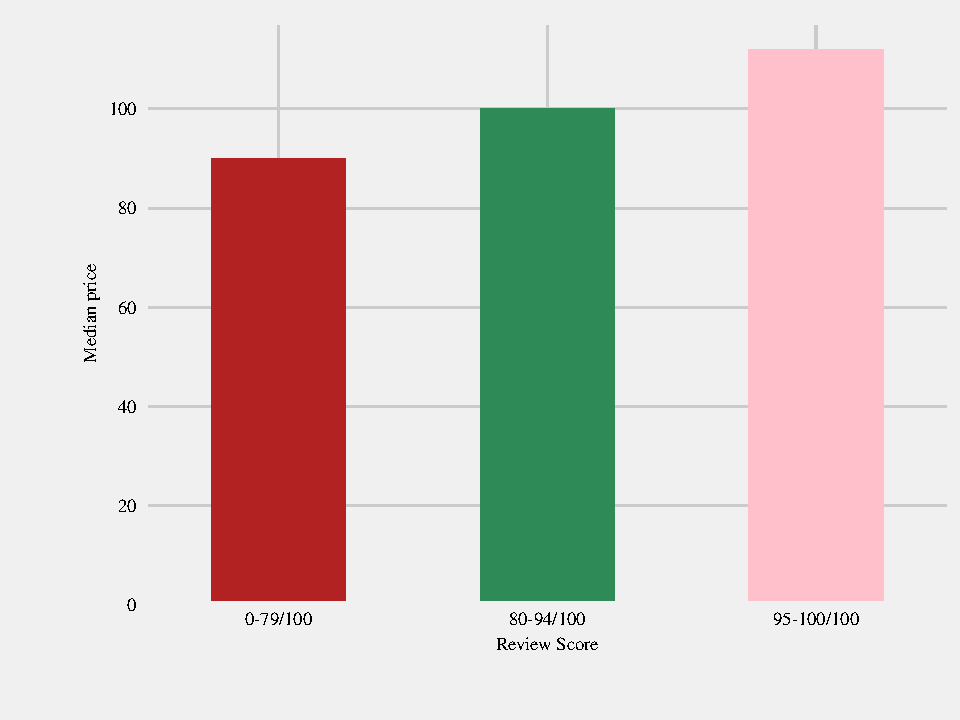
\includegraphics[width=0.85\textwidth]{median-price-by-reviews-rating.pdf}
    \caption{Median Price By Review Score Rating}
    \label{fig:price_by_review_score_rating}
\end{figure}

\subsubsection*{First and Last Review}

As can be seen from the Figure ~\ref{fig:time_since_first_review}, the most
common period in which  Airbnb listings had their first review is 2-3 years,
which means that many listings on the site have been active for at least a
couple of years. However,  fewer listings have been on Airbnb for more than four
years.

\begin{figure}[!htbp]\centering
    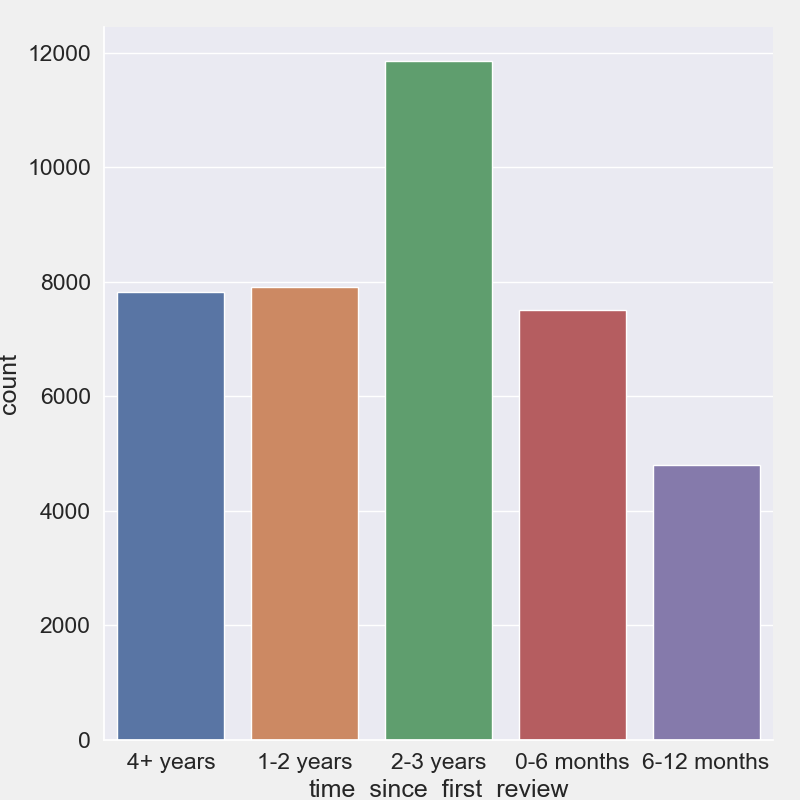
\includegraphics[width=0.7\textwidth]{Figure_15_time_since_first_review.png}
    \caption{Time Since First Review}
    \label{fig:time_since_first_review}
\end{figure}

We expect that people would pay a higher price for listing lives in Airbnb for a
long time than listings with a recent history with Airbnb.
While the rental price is higher for listings had their reviews for four years
or more, there's no difference in median price for other categories
(Figure \ref{fig:time_since_first_review_price})

\begin{figure}[!htbp]\centering
    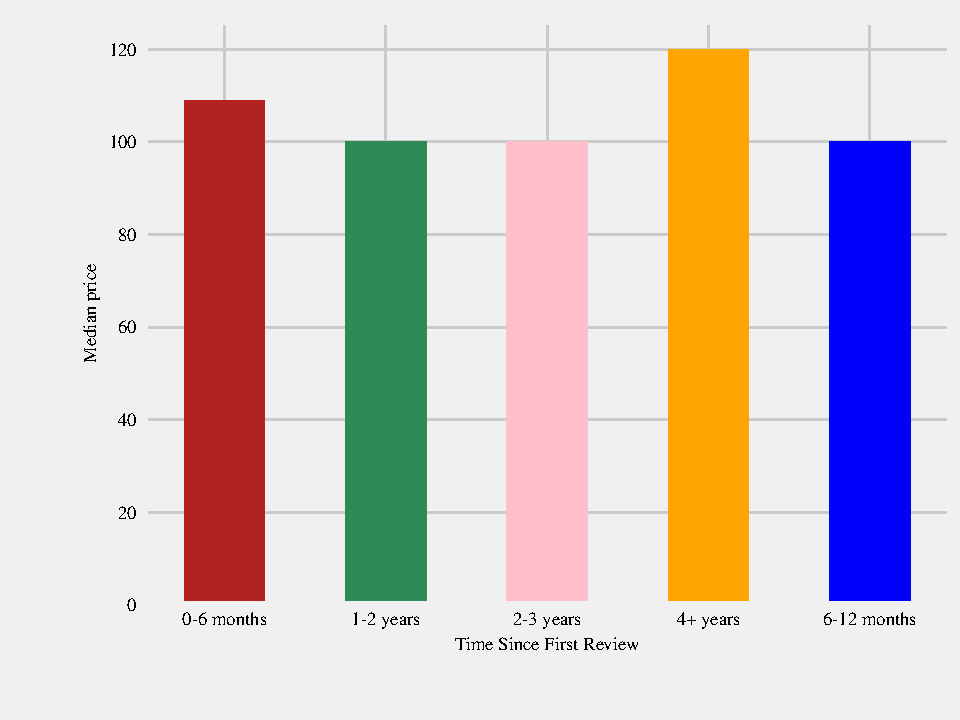
\includegraphics[width=0.9\textwidth]{median-price-by-time-since-first-review.pdf}
    \caption{Median Price By Time Since First Review}
    \label{fig:time_since_first_review_price}
\end{figure}

The bar plot ~\ref{fig:time_since_last_review} reveals that the most
common period since a listing received its last review is 2-8 weeks, which means
that many listings have been reviewed relatively recently.  What stands out in
the figure is that over 10,000 listings have not had a review for more than a
year, which means they exist on the site, but they do not have their calendars
open and are not available to reserve.

\begin{figure}[!htbp]\centering
    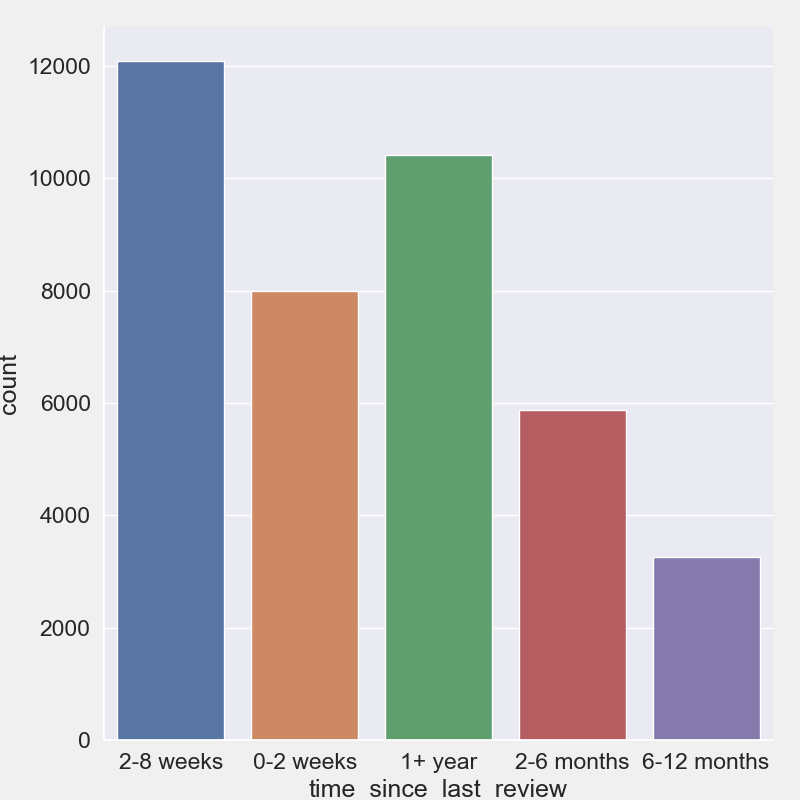
\includegraphics[width=0.7\textwidth]{Figure_15_time_since_last_review.png}
    \caption{Time Since Last Review}
    \label{fig:time_since_last_review}
\end{figure}

Time since the last review may have been an essential factor in how people
decide to rent an Airbnb listing. People may avoid booking accommodation that
has not been reviewed for a long time. Therefore, we expect the time since the
last review has a negative effect on the rental price. Contrary to our
expectation, Figure \ref{fig:time_since_last_review_price} showed no significant
difference between different categories of the number of days since the last
review.

\begin{figure}[!htbp]\centering
    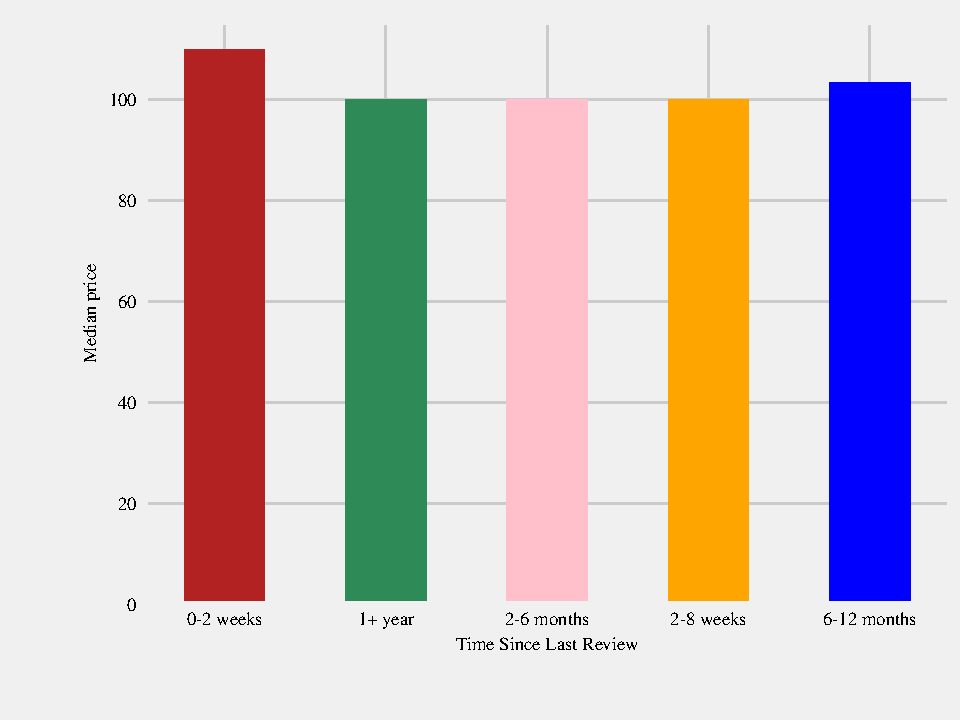
\includegraphics[width=0.9\textwidth]{median-price-by-time-since-last-review.pdf}
        \caption{Median Price By Time Since Last Review}
        \label{fig:time_since_last_review_price}
\end{figure}

\subsection{Boolean features}
\label{sec:boolean_features}

Many features (e.g. for amenities) can be true or false. This section compares
the proportions of these features that are true or false (to explore the data
and also to ascertain whether the feature is worth retaining), and the median
price of each category (to explore the relationship between the category and
price).

\subsubsection*{Superhosts}

Figure ~\ref{fig:host_is_superhost} shows that about 23\% of hosts have a
superhost badge. Hosts with superhost status usually charge higher prices. A
possible explanation for this might be that people are willing to pay a premium
price because they consider superhost status a mark of quality.  This also
accords with earlier studies(\cite{gibbs2018use},
\cite{kakar2016effects};\cite{wang2017price},\cite{cai2019price}).

\begin{figure}[!htbp]\centering
    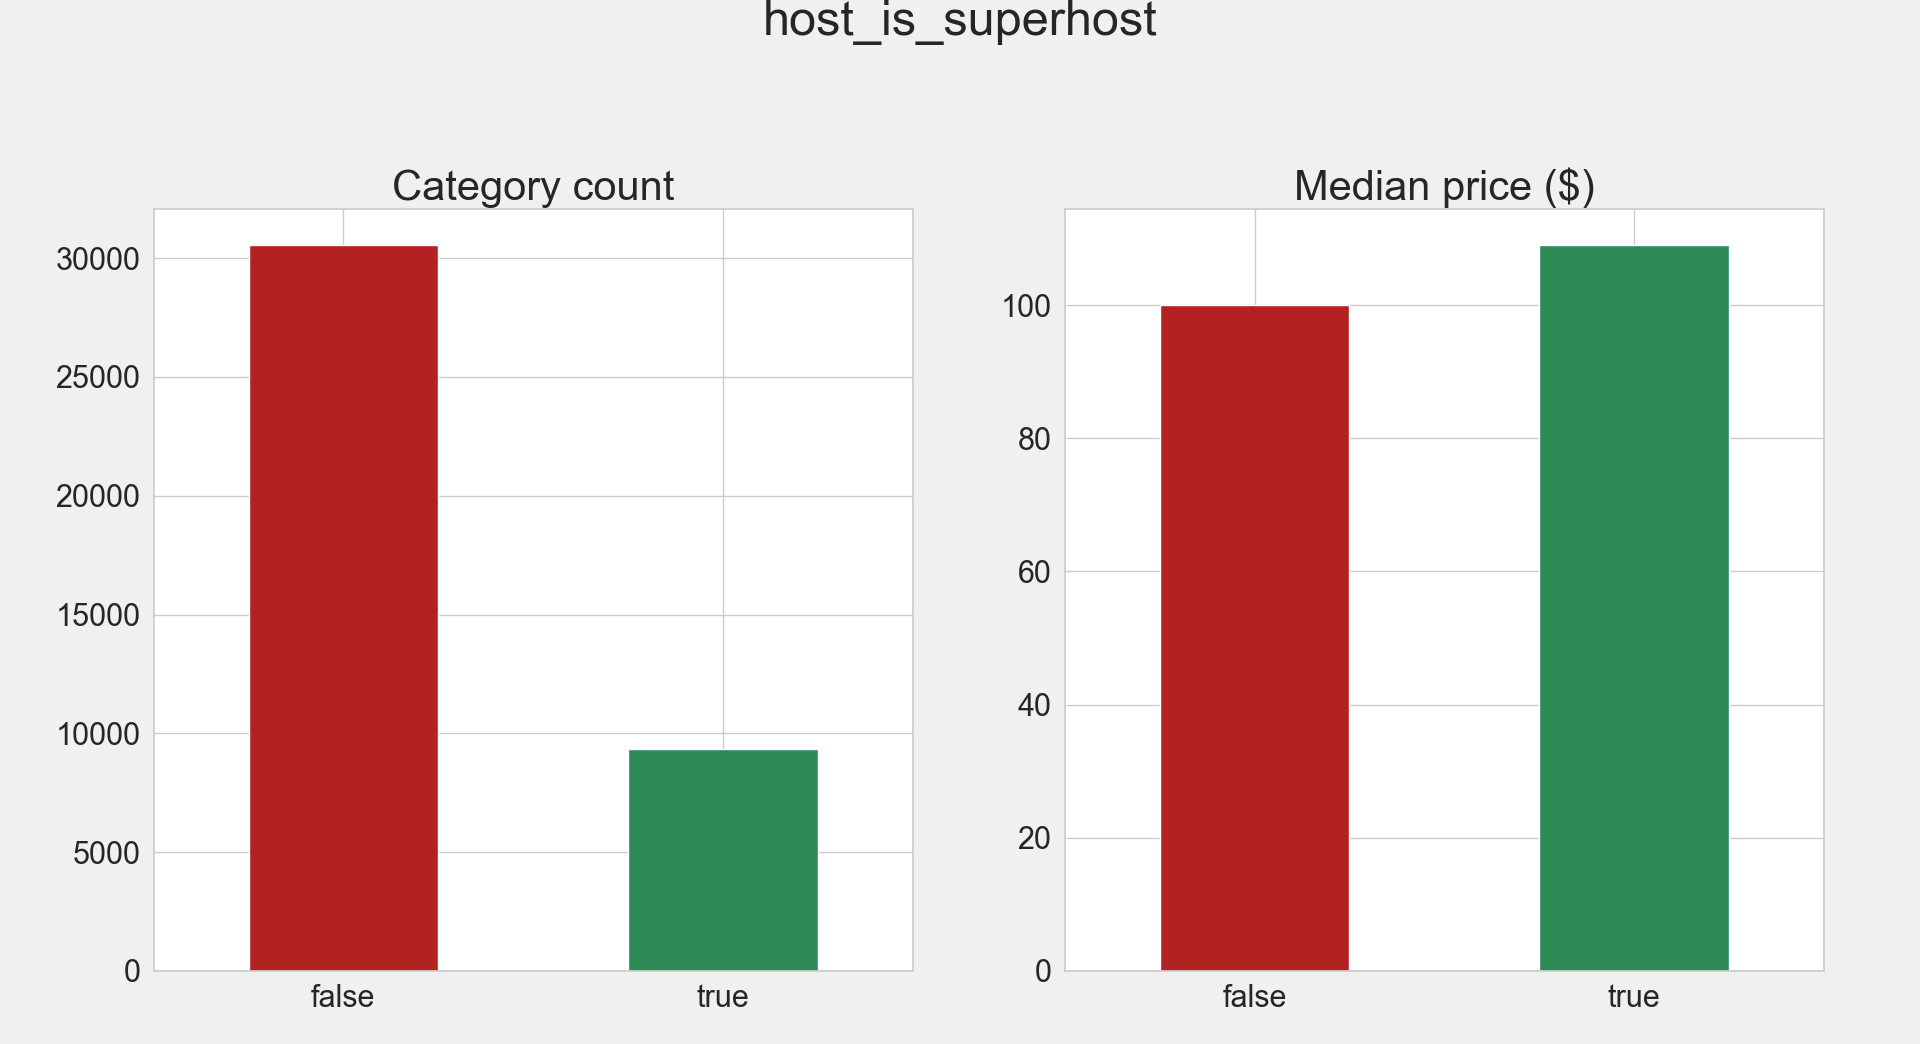
\includegraphics[width=\textwidth]{host-is-superhost.png}
    \caption{Count Plot and Median Price By Whether A Host Is a Superhost}
    \label{fig:host_is_superhost}
\end{figure}

\subsubsection*{Host verification}
In Figure ~\ref{fig:host_identity_verified}, about 49\% of hosts are verified.
Consistent with the literature (\cite{chen2017consumer}; \cite{wang2017price}),
the figure showed that hosts with verified profiles gain a price premium. The
relationship may be explained by the fact that verified profiles (e.g., by
providing ID and verifying your phone number and email address)  can increase
their trustworthiness and, therefore, can charge a higher rental price.

\begin{figure}[!htbp]\centering
    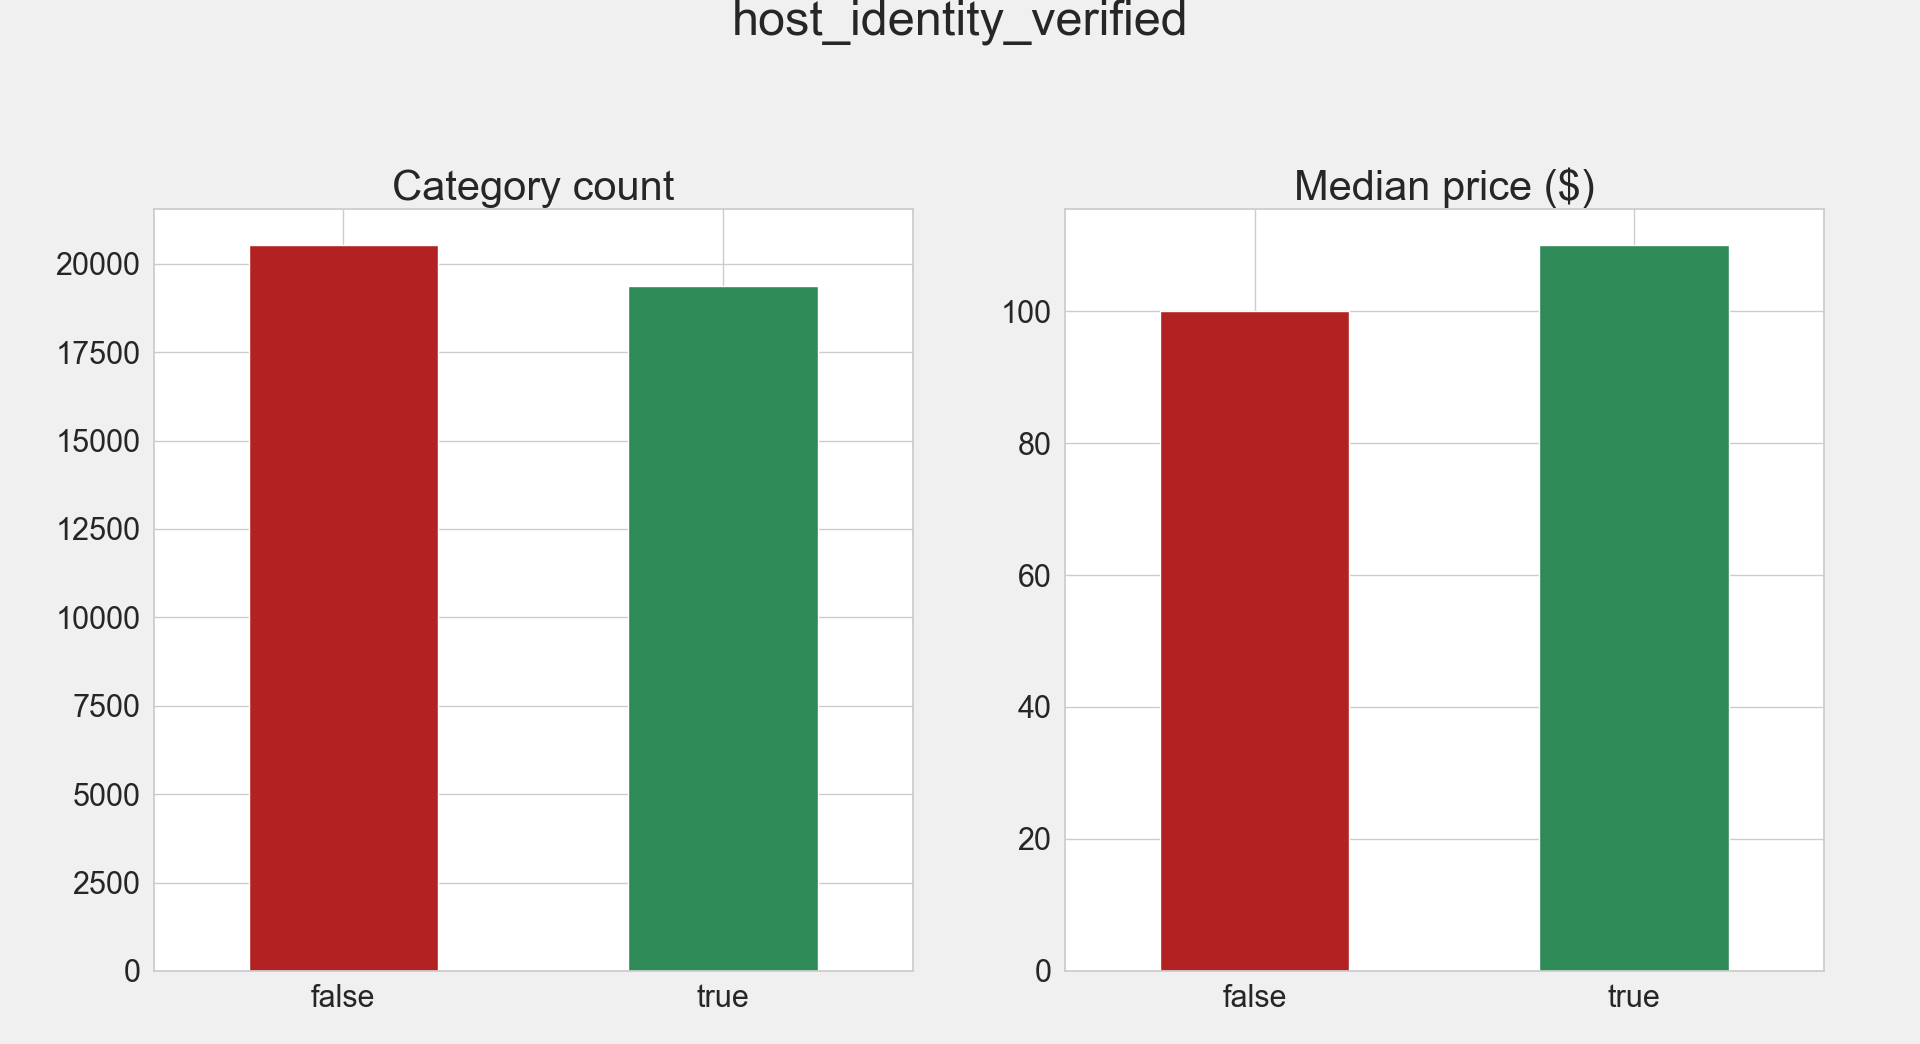
\includegraphics[width=\textwidth]{host-identity-verified.png}
    \caption{Count Plot and Median Price By Whether A Host Is Verified}
    \label{fig:host_identity_verified}
\end{figure}

\subsubsection*{Instant booking}

As shown in figure below, about 40\% of properties are instant bookable and
hosts that allow for immediate booking without confirmation  have lower prices
than those who do not. This finding seems counterintuitive, as we would expect
higher willingness-to-pay from potential guests for the added convinience of
intant booking.  This negative link can be explained by both emotional
(\textcite{wang2017price}) and economic (\textcite{benitez2018flexible}).

\begin{figure}[!htbp]
    \centering
    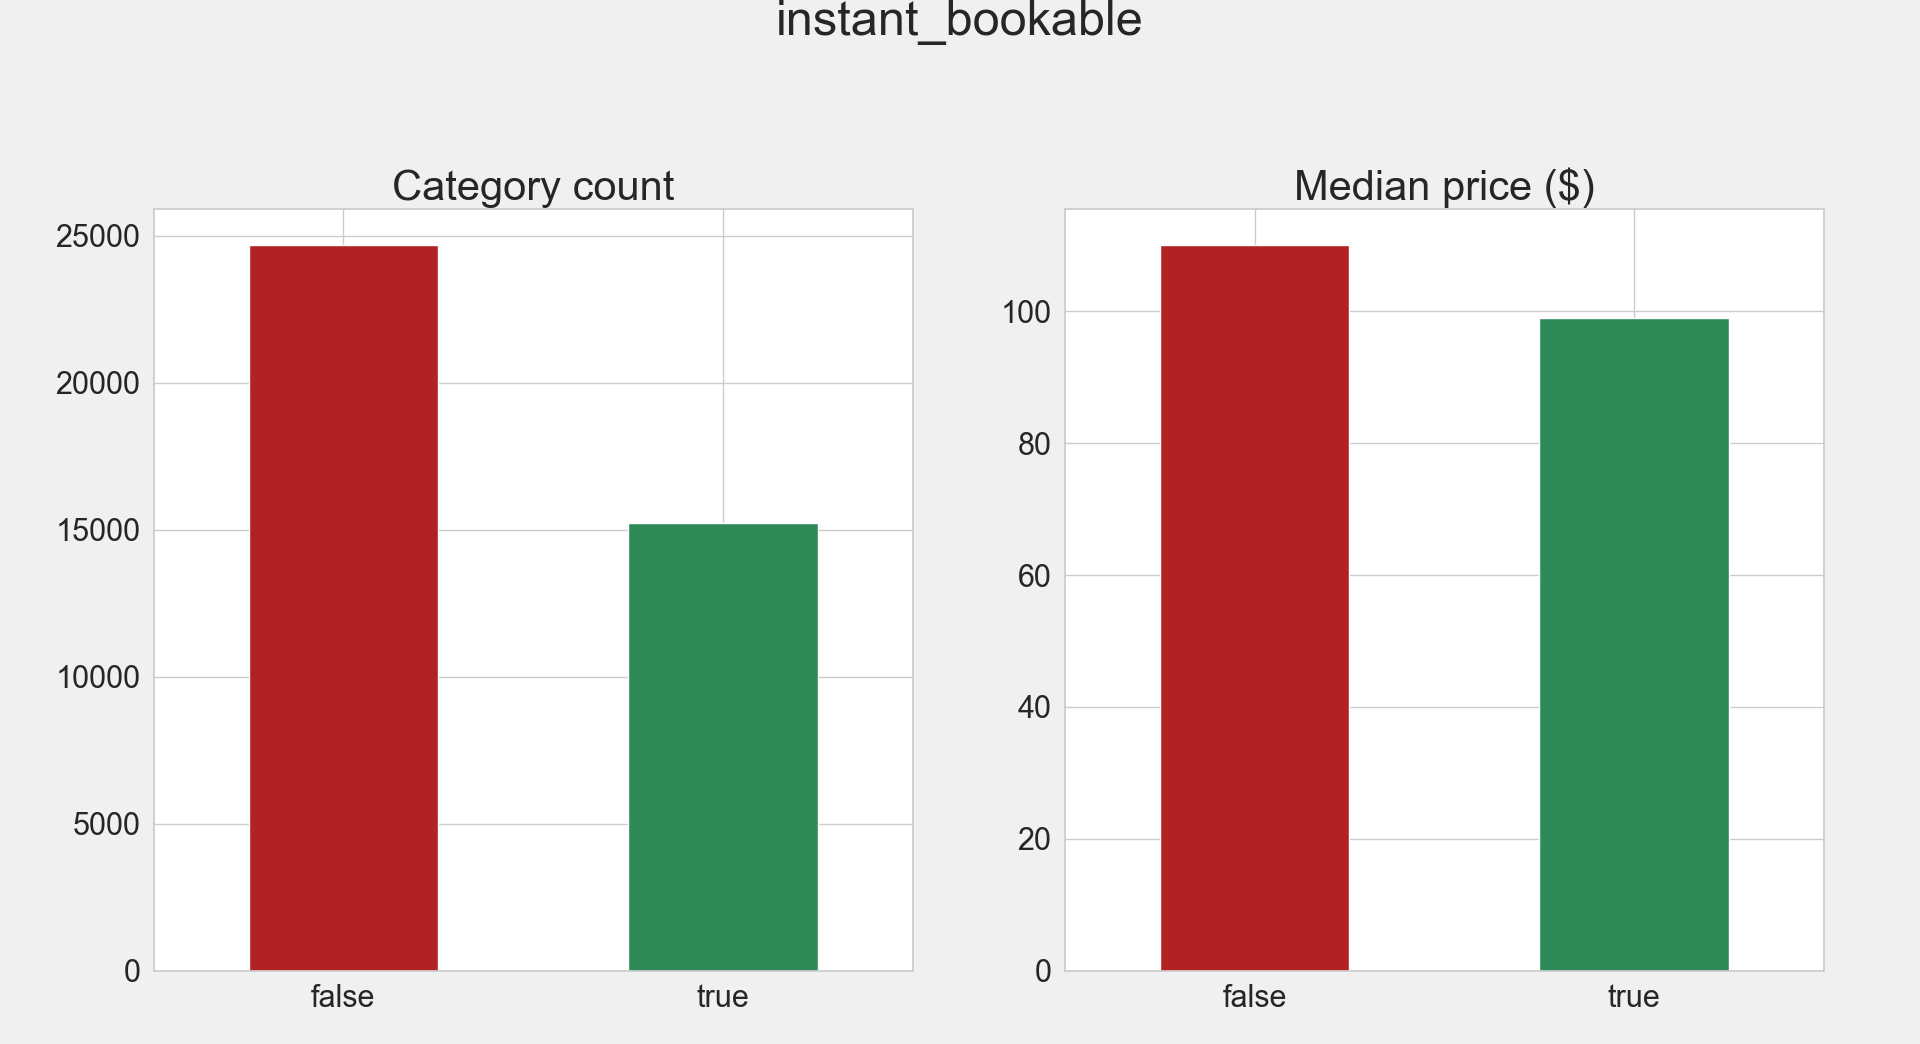
\includegraphics[width=\textwidth]{instant-bookable.png}
    \caption{instant\_bookable}
    \label{fig:instant_bookable}
\end{figure}

\subsubsection*{Amenities}

Our goal is to identify which amenities are common and which increase the price
of an Airbnb listing. We plot the count plot and each amenity's
median price to explore the relationship between the amenity and price.
Amenities then can be split into three groups:

\begin{enumerate}

  \item The first group contains uncommon amenity, but listings with it have a
    higher median price: Bed linen, Coffee machine, Basic cooking equipment,
    Elevator, Child friendly, Long term stays allowed, Private entrance, Self
    check-in, Pets allowed, Washer,dryer and/or dishwasher (white goods)
    (See
    ~\Cref{fig:elevator-and-bed-linen,fig:white-goods-and-pets-allowed,fig:self-checkin-and-coffee-machine,fig:long-term-stays-and-child-friendly,fig:private-entrance-and-cooking-basics})

  \item The second group includes common amenities and listings with it have a
      higher median price: TV, Internet, Air conditioner (See
      ~\Cref{fig:tv-and-internet,fig:air-conditioner}).

  \item The third group comprises uncommon amenities, and listings with it have
      a lower median price:  free car parking (presumably because these are less
      likely to be central properties), greeted by host. (See
      ~\Cref{fig:parking-and-host-greeting})

\end{enumerate}

It is somewhat surprising that free car parking does not have a significant
influence on the rental price. This may be because the more comfortable way and
quickest way to travel around New York City is by the subway, so people would
not consider car parking a critical factor when deciding to rent an Airbnb
listing. The reason why the host greeting does not associate with a higher price
is not apparent.

\subsection{Multivariate Exploration}
\label{sec:multivariate-exploration}

The goal of this section is to investigate the relationships between pairs of
our features. A primary concern when analyzing the relationship between various
variables is multicollinearity, a phenomenon in which two or more independent
variables substantially correlate(\textcite{cohen2013applied}).

While multicollinearity does not hurt the model's predictive
power(\textcite{kutner2005applied}), collinearity can pose problems in the
regression context. In particular,  it can be challenging to separate the
individual effects of collinear independent variables on the outcome variable.

A straightforward way to detect collinearity is to construct a correlation
matrix among predictors.  An element of this matrix that is large in absolute
value indicates a pair of highly correlated variables and are indicative of
collinearity issues.


As shown in Figure ~\ref{fig:correlation-matrix} shows the correlation matrix,
areas of multicollinearity are:
\begin{itemize}
    \item Beds, bedrooms, guests included, and the number of people that
      property accommodates are highly correlated.
    \item There are strong negative correlations between houses and apartments
        and between private rooms and entire homes.
\end{itemize}

Providing a full remedy for the multicollinearity issue is beyond the scope of
this thesis. However, we employ two  simple approaches as followed:

\begin{enumerate}
    \item The first approach is to drop problematic variables from the regression.
    \item The second method is to employ regularization techniques, which combat
        collinearity by using biased models (as demonstrated in section \ref{ssec:penalized_regression_models}),
        which reduce the error variance of estimators.
\end{enumerate}

\subsection{Time Series Analysis}
\label{sec:time_series}

We now also plotted time series charts to check for trends and seasonality.
First, we examine how long hosts have been listing properties on Airbnb in New
York.Of the Airbnb hosts that are active on the site, the first joined on 22
August 2008, and the most recent joined on 03 December 2019.
From 2011 onwards, the number of listings started growing considerably. However,
growth in the number of new hosts (of those currently listed on the site) has
decreased since mid-2014 (The trend curve in Figure
~\ref{fig:number_of_hosts_joining}).

Strong evidence of seasonality was found in  seasonal curve (Figure
~\ref{fig:number_of_hosts_joining}). The number of hosts joining Airbnb peaked in
the summer because people put properties online to utilize the increased number
of tourists in the summer holidays.


\begin{figure}[!htbp] \centering
    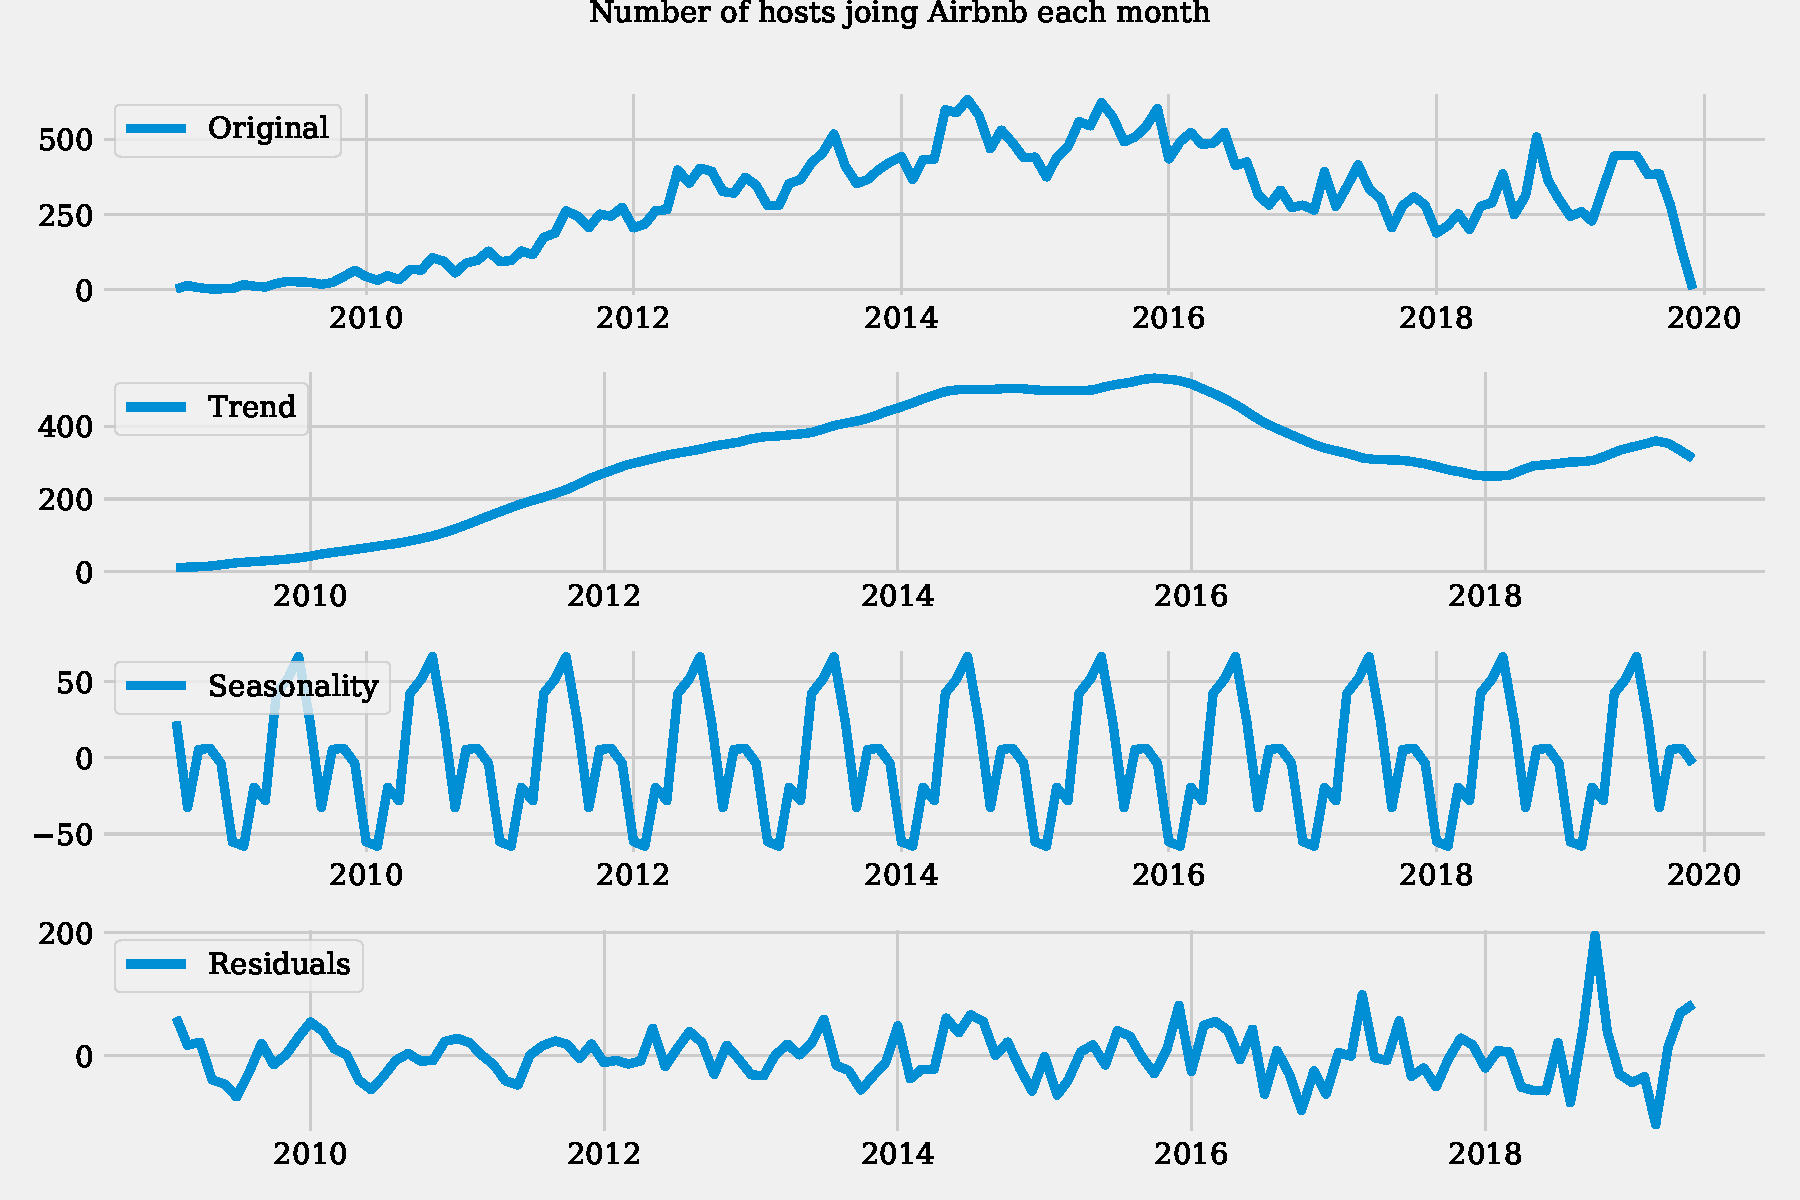
\includegraphics[width=\textwidth]{number-of-host-joining-each-month.pdf}
    \caption{Number of hosts joining Airbnb each month}
    \label{fig:number_of_hosts_joining}
\end{figure}

In terms of how prices changed over time, Figure
~\ref{fig:prices-change-by-years} shows that the average price per night for
Airbnb listings in New York has increased slightly over the
last ten years. Particularly, the top-tier property prices have increased,
resulting in a more substantial increase in the mean price than the median.


\begin{figure}[!htbp] \centering
    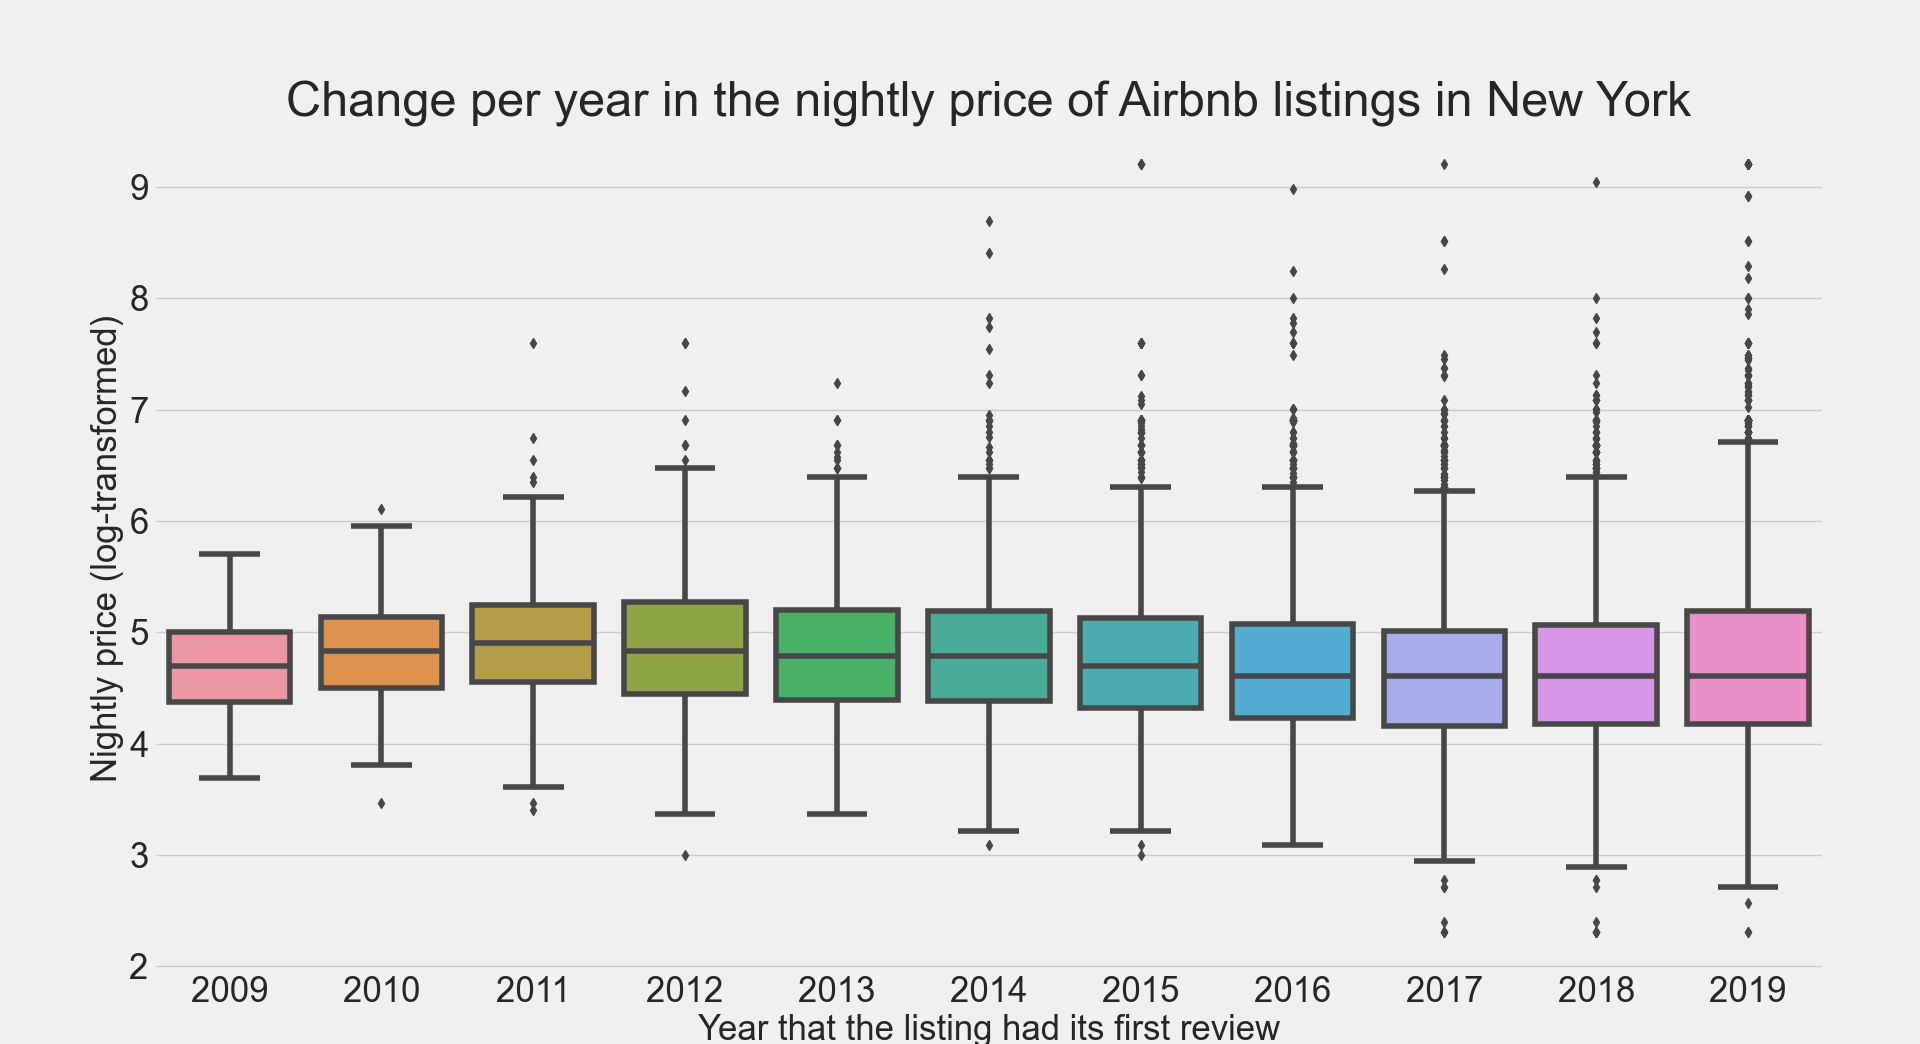
\includegraphics[width=\textwidth]{price-trend.png}
    \caption{Change per year in the nightly price of Airbnb listings in New York}
    \label{fig:prices-change-by-years}
\end{figure}


\section{Modelling}

\subsection{Training and Test Sets}
\label{sec:train_test_split}

The train-test split procedure is used to estimate machine learning algorithms'
performance when making predictions on data not used to train the model.  We
randomly split the dataset into 80\% and 20\% of listings for training and test
sets, respectively. The training set is used to fit the model, and the test
set is used to evaluate the fit machine learning model. The objective is to
estimate the machine learning model's performance on new data: data not used to
train the model.

The scikit-learn library provides an implementation of the train-test-split
procedure via the \texttt{train\_test\_split()} function.

\subsection{Findings}
\label{sec:findings}

A summary of of results is reported in Table ~\ref{tab:results}

\begin{table}[!htbp]
  \centering
  \caption{Results}
  \label{tab:results}
  \begin{tabular}{lllll}
    \hline
    ML Algorithm & Training MSE & Test MSE & Training $R^2$ & Test $R^2$ \\
    \hline
    Linear Regresion & 0.1291 &  8.5E21 &  0.7019 & -1.9E22 \\
    Ridge Regression  & 0.1291 & 0.138 & 0.7019 &  0.6857 \\
    Lasso Regression & 0.1351 & 0.1441 & 0.688 & 0.6718 \\
    XGboost &  0.0798 & 0.1173 & 0.8157 &  0.7328 \\
  \end{tabular}
\end{table}


As expected in ~\ref{linear-regression} incorporating such a large number
of features (309) makes the linear regression model overfit the data. As
shown in Table ~\ref{tab:results}, while training MSE of the linear regression
model is quite good, the model performs poorly on the test set both in terms of
in terms of $MSE$ and $R^2$.

By performing k-fold cross-validation with ten folds, we can find the tuning
parameter's value that results in the smallest cross-validation error is 115.
The test's MSE is associated with this value of  is 0.138.  The result
represents a considerable improvement of ridge regression over the test MSE we
got using least square regression.


Using cross-validation , we find the optimized penalty value $\lambda$ for lasso
is 0.005.  The associated test MSE is 0.1441, which is slightly higher than the
test set MSE of the ridge regression.  Recall from that the advantage of using
lasso regression over ridge regression is that lasso performs feature selection.
Lasso picked 153 variables while eliminated the other 125 features.


As shown by the Table ~\ref{tab:results}, XGboost consistently outperforms these
competing approaches in both mean squared error and R-squared.  With this model,
the features explain approximately 73\% of the target variable's variance and
have smaller MSE than the other regression model.

\begin{table}[!htbp]
  \centering
  \caption{XGBoost Top 20 Feature Weights}
  \label{tab:xgb-weights}
  \begin{tabular}{lr}
    \toprule
    {} &    weight \\
    \midrule
    room\_type\_Entire home/apt        &  0.336396 \\
    bathrooms                        &  0.032001 \\
    neighbourhood\_Midtown            &  0.025008 \\
    neighbourhood\_Hell's Kitchen     &  0.018545 \\
    neighbourhood\_East Village       &  0.015763 \\
    property\_type\_Other              &  0.015168 \\
    neighbourhood\_Bedford-Stuyvesant &  0.014314 \\
    neighbourhood\_West Village       &  0.014031 \\
    neighbourhood\_Chelsea            &  0.013612 \\
    neighbourhood\_Lower East Side    &  0.011874 \\
    neighbourhood\_Bushwick           &  0.011854 \\
    neighbourhood\_Upper West Side    &  0.011682 \\
    neighbourhood\_Washington Heights &  0.011659 \\
    neighbourhood\_SoHo               &  0.011582 \\
    room\_type\_Shared room            &  0.011304 \\
    neighbourhood\_Greenwich Village  &  0.010347 \\
    room\_type\_Hotel room             &  0.009697 \\
    neighbourhood\_Theater District   &  0.008575 \\
    neighbourhood\_Williamsburg       &  0.008490 \\
    neighbourhood\_Crown Heights      &  0.007979 \\
  \bottomrule
  \end{tabular}
\end{table}

Another important finding from \ref{tab:xgb-weights} was the role of location
features play in predicting price. In particular, location features located in
Manhattan and Brooklyn borough are in the top 20 important variables to predict
the price. This is consistent with what we observed in \ref{eda:neighbourhood}.
